\documentclass[12pt]{article}
\usepackage{amssymb}
\usepackage{amsfonts}
\usepackage{amsmath}
\usepackage{float}
\usepackage{rotating}
\usepackage{pdflscape}
\usepackage{setspace}
\usepackage{threeparttable}
\usepackage{fullpage}
\usepackage{rotating}
\usepackage{booktabs}
\usepackage{array,multirow}
\usepackage{epigraph}
\usepackage[round]{natbib}
\usepackage{xcolor}
\usepackage{graphicx}
\usepackage{sectsty}
\usepackage{afterpage}
\usepackage{verbatim}
\usepackage{sverb}
\usepackage{fancyvrb}
\usepackage{soul}
\usepackage{subcaption}
\usepackage{bm}

% links
\definecolor{purple}{HTML}{5601A4}
\usepackage{hyperref}
\hypersetup{
    colorlinks= true,
    allcolors = purple
}

\usepackage{etoolbox} % modify commands and many other things

% Customize Figure Font and Caption Size
\renewcommand{\figurename}{\centering\normalsize{Figure}}
\renewcommand{\thefigure}{\arabic{figure}}
\newcommand{\captionfonts}{\footnotesize}
\makeatletter  % Allow the use of @ in command names
\long\def\@makecaption#1#2{%
  \vskip\abovecaptionskip
  \sbox\@tempboxa{{\captionfonts #1: #2}}%
  \ifdim \wd\@tempboxa >\hsize
    {\captionfonts #1: #2\par}
  \else
    \hbox to\hsize{\hfil\box\@tempboxa\hfil}%
  \fi
  \vskip\belowcaptionskip}
\makeatother   % Cancel the effect of \makeatletter

% Customize Table Font
\renewcommand{\tablename}{\centering\normalsize{Table}}
\renewcommand{\thetable}{\arabic{table}}

% redefine enumerate env for closer spacing
\renewenvironment{enumerate}%
  {\begin{list}{\arabic{enumi}.}%
     {\topsep=0in\itemsep=0in\parsep=0in\partopsep=0in\usecounter{enumi}}%
   }{\end{list}}

\newlength{\Oldarrayrulewidth}
\newcommand{\Cline}[2]{%
  \noalign{\global\setlength{\Oldarrayrulewidth}{\arrayrulewidth}}%
  \noalign{\global\setlength{\arrayrulewidth}{#1}}\cline{#2}%
  \noalign{\global\setlength{\arrayrulewidth}{\Oldarrayrulewidth}}}

\renewcommand{\baselinestretch}{1.5}

\textwidth = 6.5 in
\textheight = 8.8 in
\oddsidemargin = 0.0in
\evensidemargin = 0.0in
\topmargin = 0.0 in
\headheight = 0.2 in
\headsep = 0.0 in
\parskip = 0.05in
\parindent = 0.25in

\usepackage[compact]{titlesec}
\titlespacing{\section}{0pt}{*0}{*0}
\titlespacing{\subsection}{0pt}{*0}{*0}
\titlespacing{\subsubsection}{0pt}{*0}{*0}

\renewcommand{\thesubfigure}{\Alph{subfigure}}

\sectionfont{\rmfamily\normalsize\bf}
\subsectionfont{\rmfamily\it\normalsize}
\subsubsectionfont{\rmfamily\it\normalsize}

% Set your name here
\def\emailkyle{\tt{\color{blue}kyle.butts@colorado.edu}}
\def\emailtaylor{\tt{\color{blue}taylor.jaworski@colorado.edu}}
\def\emailcarl{\tt{\color{blue}ckitchens@fsu.edu}}

% Set "thanks" indent
\makeatletter
\patchcmd\maketitle{\@makefntext}{\@@@ddt}{}{}
\patchcmd\maketitle{\rlap}{\mbox}{}{}
\makeatother

% Set footnote indent
\makeatletter
\newlength{\myFootnoteWidth}
\newlength{\myFootnoteLabel}
\setlength{\myFootnoteLabel}{.6em}%  <-- can be changed to any valid value
\renewcommand{\@makefntext}[1]{%
  \setlength{\myFootnoteWidth}{\columnwidth}%
  \addtolength{\myFootnoteWidth}{-\myFootnoteLabel}%
  \noindent\makebox[\myFootnoteLabel][r]{\@makefnmark\ }%
  \parbox[t]{\myFootnoteWidth}{#1}%
}
\makeatother

% Fix \input with tables
% \input fails when \\ is at end of external .tex file
\makeatletter
\let\input\@@input
\makeatother

\usepackage{tikz,pgfplots}
\usepackage{adjustbox}

% Commands for leaving comments \kyle{...}
\newtoggle{INCLUDECOMMENTS}
\toggletrue{INCLUDECOMMENTS}
% \togglefalse{INCLUDECOMMENTS}

\newcommand{\taylor}[1]{\iftoggle{INCLUDECOMMENTS}{{\color{magenta}\textbf{Taylor:} #1}}{}}
\newcommand{\kyle}[1]{\iftoggle{INCLUDECOMMENTS}{{\color{magenta}\textbf{Kyle:} #1}}{}}
\newcommand{\carl}[1]{\iftoggle{INCLUDECOMMENTS}{{\color{magenta}\textbf{Carl:} #1}}{}}


\begin{document}  
\begin{titlepage}

\title{\singlespacing {\LARGE The Urban Wage Premium in Historical Perspective}\thanks{This version of the paper includes preliminary results. Please do not cite without permission.}}
\author{%
  \large Kyle Butts\thanks{University of Arkansas, Department of Economics, ({\emailkyle})}
  \and
  \large Taylor Jaworski\thanks{CU-Boulder, Department of Economics, and NBER ({\emailtaylor})}  
  \and
  \large Carl T.
  Kitchens\thanks{Florida State, Department of Economics, and NBER ({\emailcarl})}  
}
\date{\large \today}

\maketitle

\begin{singlespacing}
\begin{abstract}\noindent
We estimate the urban wage premium in the United States from 1940 to 2010.
Drawing on recent advances in the literature on selection on unobservables, we show how to control for heterogeneity in the characteristics of individuals that choose to live in cities to address endogenous sorting.
Estimates from naive comparisons of individuals living in urban versus rural areas substantially overstate the urban wage premium.
We find that the premium is highest in the middle of the twentieth century (about 12 percent in 1940 and 1950) relative to the early in twenty-first century (declining to a few percent by mid-2020).
Overall, the urban wage premium is decreasing and sorting explains a larger fraction of the difference in urban versus rural earnings across our sample period.
\end{abstract}
\end{singlespacing}

\thispagestyle{empty}

\end{titlepage}


%%%%%%%%%%%%%%%%%%%%%%%%%%%%%%%%%%%%%%%%%%%%%%%%%%%%%%%%%%%
\section{Introduction}
%%%%%%%%%%%%%%%%%%%%%%%%%%%%%%%%%%%%%%%%%%%%%%%%%%%%%%%%%%%

The average U.S. worker living in an urban area in 2010 earns 35 percent more than their non-urban counterparts.\footnote{
We use the 2010 ACS estimates to compute the average annual wage for individuals living in MSAs and outside of MSAs based on individuals that are in the labor force, report non-negative wage income, and who are not missing wage income data.} 
This pattern of higher average wages in cities holds across the globe and through out the past 80 years \citep{Boustan_Bunten_Hearey_2013}.
% motivatig a large literature in urban economics to understand the drivers of the urban wage gap. 
The fact that wages are higher in cities cannot be interpreted as the causal effect of cities due to the potential for non-random sorting of people or firms into cities based on preferences, skills, or productivity.\footnote{
For example, positive selection on the firm side may come from more productive firms paying higher wages, and only high-productivity firms locating and surviving in cities where larger markets induce tougher competition.} 
Is the difference driven by increased productivity stemming from agglomeration economies or high-ability workers sorting into urban areas \citep*[e.g.][]{behrens2014productive,moretti2011handbook,puga2010magnitude}?
Empirical evidence focused in the last 30 years has found a large portion of the observed wage premium is driven by non-random sorting, but a true effect of urbanity on wages still exists.

This paper asks how has selection and the true causal wage-benefits of urban living has changed over time. 
Past research shows that the observed raw differences in wages between urban and non-urban workers was around 35 percent in 1940, decreasing by one-third to one half in 1980 to 20-25 percent, and increasing again to 35 percent by 2010 \citep*{dauth2022matching,Boustan_Bunten_Hearey_2013}. 
However, no estimates exist prior to 1990 on whether this is due to changes in sorting patterns or changes to the causal returns to urbanity.
Given the role of agglomeration in economic models of cities, regions, and national growth, it is important to understand long run changes in the causal effect of cities on wages. 
Moreoer, understanding how the underlying drivers of selection and strength of agglomeration forces have varied over time is important for predicting the success of place-based policies \citep[e.g.][]{kerr2020tech} or to understand growth trajectories in the context of endogenous growth models \citep[e.g.][]{martin2001growth}. 
% recent work shows that the difference between urban and non-urban wages has roughly doubled since 1980 \citep*{dauth2022matching}.

% While the literature has not estimated causal effects for earlier periods, \citet*{Boustan_Bunten_Hearey_2013} provide descriptive evidence for the United States going back more than a century.
% Their key finding is a U-shaped pattern since 1940: the observed difference between urban and non-urban wages is approximately 35 percent in 1940, decreases to between 20 and 25 percent until 1980, and has since returned to be above 35 percent. 
% In particular, the key identification challenge arises in disentangling the productivity effect of cities from unobserved characteristics of individuals, firms, or cities induced by endogenous sorting. 

Research in this area has typically addressed these concerns using detailed worker- and firm-level panel data.
Comparing the same individuals before and after moving to an urban area removes time-invariant wage variation due to worker characteristics, such as ability.
Then, the remaining gap or subsequent wage growth between urban and rural earnings is attributed to agglomeration forces stemming from knowledge sharing, improved firm-worker matching, human capital accumulation, labor market pooling, or input-output linkages \citep*{BaumSnow_Pavan_2012,Combes_Duranton_Gobillon_2008, dauth2022matching, Glaeser_Mare_2001,gould2007cities,Yankow_2006}.
The previous literature provides a range of estimates regarding the urban wage premium.
For example, \citet*{Glaeser_Mare_2001} estimate an urban wage premium between 4.5 and 11 percent after controlling for individual characteristics and, more importantly, unobserved heterogeneity with worker-specific fixed effects. \citet{gould2007cities} finds a premium of 11.5 percent for white-collar workers and a smaller premium of 1.2 percent for blue-collar workers.\footnote{
\citet{rosenthal2004evidence} and, more recently, \citet{diamond2021spatial} survey the large literature that describes the theoretical underpinnings and empirical findings related to agglomeration and urban sorting.}

Due to limited data availability the existing literature has focused primarily on the last three decades and little is known about the evolution of the urban wage premium before 1980.
The primary challenge is that census data only provides a cross-sectional snapshot of who lives in an urban area and how much they earn, preventing the standard strategy of tracking workers when they move into or out of an urban area. 
Hence, any cross-sectional estimates comparing urban to non-urban workers will be confounded by unobserved worker characteristics that drive sorting.

In this paper, we show how to use readily available census data to estimate the urban wage premium while controlling for observed individual characteristics as well as unobserved characteristics following the approach in \citet*{altonji2018estimating}.
Their setup is based on the classic urban location choice model. 
Workers vary in their willingness to pay for location-specific amenities based on observable and, importantly, \emph{unobservable} characteristics.
% Workers then  draw location-specific idiosyncratic errors (assumed to be distributed type-1 extreme value). 
% The choice model gives rise to create two important mappings. 
Because of differences in willingness-to-pay, location-specific averages of observable characteristics vary based on a location's underlying amenities. 
Similarly, the averages of unobservable characteristics vary because of (potentially different) location-specific amenities. 
If the amenities driving both observable and unobservable sorting are the same, the model suggests that controlling for observable location-specific averages is sufficient to control for unobservable averages.\footnote{
  We discuss this assumption below and provide evidence that builds confidence in the plausibility.
}
This approach is crucial as it allows us to address sorting when estimating the historical urban wage premium without individual-level longitudinal data.

We estimate the urban wage premium from 1940 to 2010.\footnote{
  Specifically, we use only repeated cross-sections from the US decennial censuses and American Community Survey beginning in 1940 when information on individual wages was first reported.
}
Focusing first on the period since 1980, where we can make direct comparisons to the existing literature, we document an urban wage premium starting at 7.7 percent in 1980 and declining to around 5 percent in the following decades.
This is consistent with the results reported in \citet*{Glaeser_Mare_2001}, \cite*{Yankow_2006}, and \citet*{BaumSnow_Pavan_2012} and provides support that our approach (drawing on \citet*{altonji2018estimating}) addresses the key identification concern related to sorting.
Second, moving to earlier decades, we estimate an urban wage premium of 12.9 percent in 1940, 16.2 percent in 1950, 13.3 percent in 1960, and 9.2 percent in 1970. % Exponentiate table 3
% \kyle{Check these numbers}
The pattern suggests that agglomeration forces were relatively more important prior to 1980, although sorting still drives a large portion of the observed premium between 1940 and 1980.\footnote{
  Due to changes in the definition of cities over time (smaller cities being added over-time), we also estimate the urban wage premium on consistent set of locations based on the urban status in 1940. 
  The results remain very similar.
}

We find that the causal urban wage premium, which reflects the fact that workers moving to cities earn more, was large in 1940 but steadily declined over time, reaching its lowest point by 2010, the most recent year in our data. 
This pattern aligns with several well-documented trends in the literature. 
First, the increasing role of sorting in explaining the wage differential between urban and non-urban areas is consistent with the rising migration of highly educated workers to cities \citep*{shapiro2006smart, moretti2013real, Diamond_2016}. 
Though raw wage premiums have been growing in recent years, this migration and our results suggest this is a compositional effect rather than a growth in the causal premium. 
This trend is also linked to structural changes in manufacturing after 1950 \citep*{dumais2002geographic, glaeser2010did}, which contributed to shifting economic activity toward urban areas. 
Historically, cities were manufacturing hubs with large agglomeration forces which enhanced worker's productivity. 
The shift away from manufacturing in cities could be a driver of the decline in the causal wage premium. 
Moreover, the increased mobility of highly skilled workers in response to tax policy further supports these findings \citep*{moretti2017effect, verginer2021talent, akcigit2016taxation}.

\kyle{We have these, but not sure where to put them}
Another contributing factor is the growing body of evidence that highly skilled workers are increasingly sorting into cities based on improved local amenities \citep*{baum2020accounting, Diamond_2016, su2022rising, glaeser2001consumer, glaeser2003urban, glaeser2009wealth}. 
\footnote{
  Our results are also consistent with a growing literature that emphasizes the potential to overstate agglomeration effects in small samples \citep*{ahlfeldt2022granular, dingel2020spatial, schoefer2022productivity}. 
  For instance, \citet*{schoefer2022productivity} show that as much as three-quarters of the variation in regional productivity dispersion may be due to small sample bias. Likewise, \citet*{dingel2020spatial} illustrate that when accounting for granularity, the potential impacts of Amazon's HQ2 are smaller compared to predictions from traditional spatial equilibrium models.
}

The first concern with our results is that while urban workers might earn more in wages, they also face larger housing costs and hence there might not be a \emph{real} benefit to urbanity after adjusting for housing costs.
We calculate a wage meausre that subtracts off housing costs following \citet{ganong2017has}, and reestimate both the raw and causal (net-)wage premium. 
After adjusting for housing costs, the raw wage premium is decreased significantly between around 18\% in recent years and . 
The decline is smallest around 1970 with around a 5 percentage point decline and larger at the beginning and end of our sample with around 15 percentage point decline. 
However, our causal estimates remain roughly unchanged. 
There is a 3-4 percentage point decline in 1940 and 1950, but otherwise our estimates remain stable. 
\kyle{This is likely due to the fact that \emph{rent} is an amenity that people sort on and we absorb that impact already.}

In addition to the main findings, we explore several potential sources of heterogeneity.
First, we examine changes in the urban wage premium across the distribution of city sizes.
To do so, we estimate wage premiums separately for the 20 largest urban areas (based on 1940 populations) and other urban areas.
We show that in 1940, the largest cities had larger urban wage premiums relative to smaller urban areas.
However, the gap has narrowed since the 1980s.
The pattern we document is consistent with the transition of cities from heavy manufacturing bases to idea-generating locations.

Second, we consider regional differences and confirm that urban wage premium is falling \textit{within} each region.
The consistent fall of the premium within each region suggests that it is not changes in regional development (i.e., the deindustrialization of the North and rise of the Sunbelt) driving changes in the urban wage premium.
We do find important regional trends that are consistent with the historical narrative.
The Midwest had the largest urban wage premia in the middle of the century (around 25\% in 1950) that could reflect the strong agglomeration forces of manufacturing employment. 
The west has had a growth in estimated urban wage premium since 1990, perhaps picking up on the growth of the technology sector in Silicon Valley and other regions. 

Third, we estimate urban wage premium for college and non-college educated workers. 
We find that throughout our sample, the urban wage premium is higher for college-educated workers.
This is consistent with the complentary between skilled workers and cities emphasized by \citet{moretti2013real}.

Fourth, we estimate urban wage premium separately for Black and White workers. 
In all years, the premium for Black workers is no smaller than for White workers and is particularly larger between 1950 and 1970.
The Black urban wage premium is estimated to be five to ten percentage points larger in the middle of the 20th century which is in line with the timing of the Great Migration \citep{derenoncourt2022can}.

Fifth, we try to understand the role of urban \emph{wage-growth} premium as first documented by \citet{BaumSnow_Pavan_2012}. 
We are fundamentally limited by cross-sectional data and can not observe directly whether a worker's wage grows faster in an urban area. 
However, we estimate separate wage premia for older and younger workers assuming that the former has more years of urban experience and should presumably have larger wage premia.
We indeed find that older workers have higher premia in most years, but the gap shrinks to zero in later years. 


Finally, we provide evidence that the decline in the urban wage premium is consistent with the pattern of national wage compression documented by \citet{goldin1992great}.
\kyle{Do we think we should still include this?}



%%%%%%%%%%%%%%%%%%%%%%%%%%%%%%%%%%%%%%%%%%%%%%%%%%%%%%%%%%%%%%%%%%%%%%%%%%%%%%%%
\section{Data and Summary Statistics}\label{sec:data}
%%%%%%%%%%%%%%%%%%%%%%%%%%%%%%%%%%%%%%%%%%%%%%%%%%%%%%%%%%%%%%%%%%%%%%%%%%%%%%%%

% Need to say something about what locations are in this section
In this section, we describe the data we use to estimate the urban wage premium and key empirical patterns regarding the changes in urbanization, education, and the urban versus non-urban wage difference in the second half of the twentieth century.
First, we draw on publicly available data covering the period between 1940 and 2010 \citep{ruggles2022full, ruggles2022census}.
For 1940, we use the complete count of the US Census to measure the average earnings per worker for wage earners.
For 1960 and 1970, we use the 5 percent samples of the census.
For 1950, 1980, 1990, and 2000, we draw on the 1 percent samples of the census.
Finally, for 2010, we use the American Community Survey.
In each year, we restrict the data to include adult males living in the continental US between the ages of 25 and 65 who report being employed for at least 26 weeks in the sample year.
We use person weights to calculate summary statistics and estimate regressions. 

To construct average weekly earnings, we divide the reported total income by the number of weeks worked in the survey year.\footnote{
  For individuals earning the top income code, we set their total income to the lower top income cutoff multiplied by $1.5$.
  These cutoffs are reported in the IPUMS documentation for the \texttt{INCWAGE} variable.
  In 2015 dollars, the cutoffs are \$84,500 for 1940, \$99,2000 for 1950, \$199,500 for 1960, \$309,000 for 1970, and \$225,000 for 1980.
  Afterward, IPUMS reports income as the median wage above that year's cutoff.
  Results are robust to dropping all individuals earning the top income code. 
  \kyle{Add this file back into the replication code.}
} 
We then convert all earnings to 2015 dollars using the Consumer Price Index.
Since housing costs are higher in urban areas, we construct a measure of `real wages' following \citet{ganong2017has}. To do so, we use either (i) five percent of the reported housing value or twelve times the reported monthly rent and divide by 48 to get the weekly housing costs. We winsorize the estimated housing cost at the first and 99th percentiles and subtact this from the weekly wages.\footnote{
  Since 1950 does not have microdata on rent, we use the average rent from the Census tables.
  % In addition, we drop workers with negative weekly net-of-housing-costs wages. \kyle{Check this}
} 

In addition to wages, across all samples, consistent information is available on whether the individual is living in an urban area (metropolitan statistical area), age, educational attainment, and race.
We use this information to construct the individual- and group-level controls for our empirical analysis.
We assign workers to a city based on the metropolitan statistical area (MSA) in which they reside; workers not living in a city are assigned to their state of residence. 

We begin by describing a few key empirical patterns in Table \ref{tab:summ}.
First, we report the raw observed difference between urban and rural wages in column 2.
Here we document a clear U-shape in the summary statistics.
The urban wage gap started at 31.3 percent in 1940 and declined sharply through 1980.
Beginning in 1980, the urban wage gap increased until 2000 where it reached nearly the same level as reported in 1940.
Next, in column 3, we report the share of the population living in urban locations each year.
In 1940, 66 percent of individuals lived in urban areas.
By 2010, the urban share increased to 79.4 percent.
The pattern of increasing urbanization is consistent with prior literature such as \citet{moretti2013real} and \citet{Boustan_Bunten_Hearey_2013}.
To highlight the potential role of sorting, the remaining columns provide information the overall fraction of the population with college degree in each year and differences in this share across urban and non-urban areas.
From column 4, the share of the population with a college degree increased over time.
From columns 5 and 6, the share of the population with a college degree increases in both urban and rural areas over time; however, the share rises faster in cities.
Together, the trends in Table \ref{tab:summ} highlight that since 1940 cities have become more populated and more educated relative to rural areas, which suggests increased sorting based on skills.
The goal of the empirical approach is to address the potential role of changes in the extent of sorting based on education, other demographic characteristics, and unobserved productivity over time.  

%%%%%%%%%%%%%%%%%%%%%%%%%%%%%%%%%%%%%%%%%%%%%%%%%%%%%%%%%%%%%%%%%%%%%%%%%%%%%%%%
\begin{table}[t]
  \caption{Summary Statistics}
  \label{tab:summ}
  \renewcommand{\arraystretch}{1.25}

  \resizebox{\columnwidth}{!}{

  \begin{threeparttable}
    \begin{tabular}{@{} c @{\extracolsep{20pt}} c @{\extracolsep{5pt}} cccc @{}}
      % Head
      \toprule

      & & & \multicolumn{3}{c}{\% With College Degree} \\
      \cmidrule{4-6}
      Year & \multicolumn{1}{c}{\% Wage Gap} & \multicolumn{1}{c}{\% Urban} & \multicolumn{1}{c}{Overall} & \multicolumn{1}{c}{in Urban Areas} & \multicolumn{1}{c}{in Non-urban Areas} \\
      (1) & \multicolumn{1}{c}{(2)} & \multicolumn{1}{c}{(3)} & \multicolumn{1}{c}{(4)} & \multicolumn{1}{c}{(5)} & \multicolumn{1}{c}{(6)} \\  

      % Body
      \toprule

      1940 & 31.3 & 66.0 & 8.4 & 8.8 & 7.6 \\
1950 & 21.9 & 68.7 & 8.0 & 8.6 & 6.7 \\
1960 & 23.6 & 65.6 & 11.6 & 12.9 & 9.1 \\
1970 & 23.6 & 74.7 & 16.6 & 17.8 & 13.0 \\
1980 & 19.9 & 72.8 & 24.2 & 26.6 & 17.5 \\
1990 & 25.6 & 73.5 & 28.0 & 31.1 & 19.6 \\
2000 & 31.4 & 78.7 & 30.5 & 33.4 & 19.8 \\
2010 & 30.1 & 79.4 & 33.5 & 36.4 & 22.2 \\


      \bottomrule
    \end{tabular}
        
    % Notes 
    \begin{tablenotes}\footnotesize
        \item\noindent\textit{Notes.} This table presents summary statistics for the final ACS sample.
The data cleaning process is described in Section \ref{sec:data}.
    \end{tablenotes}
  \end{threeparttable}

  }
\end{table}
%%%%%%%%%%%%%%%%%%%%%%%%%%%%%%%%%%%%%%%%%%%%%%%%%%%%%%%%%%%%%%%%%%%%%%%%%%%%%%%%

The geography of high-wage urban centers has also changed over time.
Table \ref{tab:top} reports the ten urban areas with the highest urban wage differences in 1940 and 2010.
In particular, we calculate the difference in the average log wage in an urban and non-urban area.
While several of the cities are among the highest paying in both 1940 and in 2010 (i.e., San Francisco, Washington, D.C., San Jose, Seattle), centers of manufacturing in the industrial North and Midwest (i.e., Flint, MI, Detroit, MI, Lansing, MI, Chicago, IL, Rochester, NY) have lost their prominence in favor of cities closely associated with high-tech manufacturing.
This descriptive pattern reflects the combination of several changes in the US economy since 1940.
The main goal of remainder of the paper is to quantify and better understand changes in the urban wage premium over time and the relative importance of agglomeration (i.e., the causal effect of cities) versus sorting. 

%%%%%%%%%%%%%%%%%%%%%%
\begin{table}[t]
  \caption{Top Ten Cities by Urban Wage Premium in 1940 and 2010}
  \label{tab:top}
  \renewcommand{\arraystretch}{1.25}

  \resizebox{\columnwidth}{!}{
  \begin{threeparttable}
    \begin{tabular}{@{} lr @{\extracolsep{20pt}} l @{} r @{}}
      % Head
      \toprule

      \multicolumn{2}{c}{1940} & \multicolumn{2}{c}{2010} \\
      \cmidrule{1-2} \cmidrule{3-4} 
      Name & Premium & Name & Premium \\
        

      % Body
      \toprule

Flint, MI & 47.9\% & San Jose-Sunnyvale-Santa Clara, CA & 63.2\% \\ 
Detroit, MI & 46.0\% & Bridgeport-Stamford-Norwalk, CT & 54.7\% \\ 
Washington DC, MD/VA/WV & 45.7\% & San Francisco-San Mateo-Redwood City,CA & 52\% \\ 
San Francisco, CA & 44.0\% & Washington-Arlington-Alexandria DC-VA & 42.9\% \\ 
Seattle-Everett, WA & 41.7\% & Boston-Quincy, MA & 42.7\% \\ 
Lansing-East Lansing, MI & 41.0\% & Seattle-Bellevue-Everett, WA & 42.2\% \\ 
New York, NY & 40.2\% & Santa Cruz-Watsonville, CA & 36.7\% \\ 
Sacramento, CA & 39.2\% & Trenton-Ewing, NJ & 36.1\% \\ 
Chicago, IL & 38.8\% & Midland, TX & 34.0\% \\ 
Rochester, NY & 38.1\% & Baltimore-Towson, MD & 33.6\% \\ 
    

      \bottomrule
    \end{tabular}
        
    % Notes 
    \begin{tablenotes}\footnotesize
        \item \textit{Notes.} This table presents the top ten cities in terms of observed wage premia relative to non-urban areas.
    \end{tablenotes}
  \end{threeparttable}
  }

\end{table}
%%%%%%%%%%%%%%%%%%%%%%

%%%%%%%%%%%%%%%%%%%%%%%%%%%%%%%%%%%%%%%%%%%%%%%%%%%%%%%%%%%
\section{Measuring the Urban Wage Premium}
%%%%%%%%%%%%%%%%%%%%%%%%%%%%%%%%%%%%%%%%%%%%%%%%%%%%%%%%%%%

We begin by estimating the urban-rural wage difference in a simple regression framework.
We follow the literature by adding individual-level covariates to address sorting into urban locations.
In particular, we estimate the following equation separately for each year:
\begin{equation}\label{eq:controls}
    \log(\text{wage}_i) = \beta_0 + \beta_1 \text{urban}_i + \bm{X}_{i} \delta + \varepsilon_i,
\end{equation}
where $\text{wage}_i$ is average weekly earnings and $\bm{X}_i$ is a set of control variables consisting of indicator variables for five-year age bins, educational attainment dummy variables, and an indicator for race (white versus non-white).\footnote{
  We are limited in our control variables beacause we want these to remain constant across census years.
}
Our estimate of $\beta_1$ is the average premium in percentage terms that urban workers earn relative to non-urban workers (in figures we use percent by calculating $e^{\hat{\beta}_1} - 1$).
Without controls, the coefficient reflects the mean difference in earnings between individuals living in urban and non-urban locations.
If the set of control variables fully accounts for sorting, we could interpret $\beta_1$ as the causal effect of living in an urban location on earnings.
However, there are several reasons individuals sort into cities that are not captured by their observable characteristics.
For example, individuals with certain attributes may sort to cities because they value specific consumptive amenities, such as entertainment or dining.
If these sorting patterns are correlated with productivity, $\beta_1$ would suffer from omitted variables bias.
As a result, the estimated $\beta_1$ should be interpreted as a correlation. 

%%%%%%%%%%%%%%%%%%%%%%
\begin{figure}[t]
  \caption{Urban Wage Premium Controlling for Individual Characteristics, 1940-2010}
  \label{fig:premium_over_time}
  \begin{adjustbox}{width=\textwidth,center}
    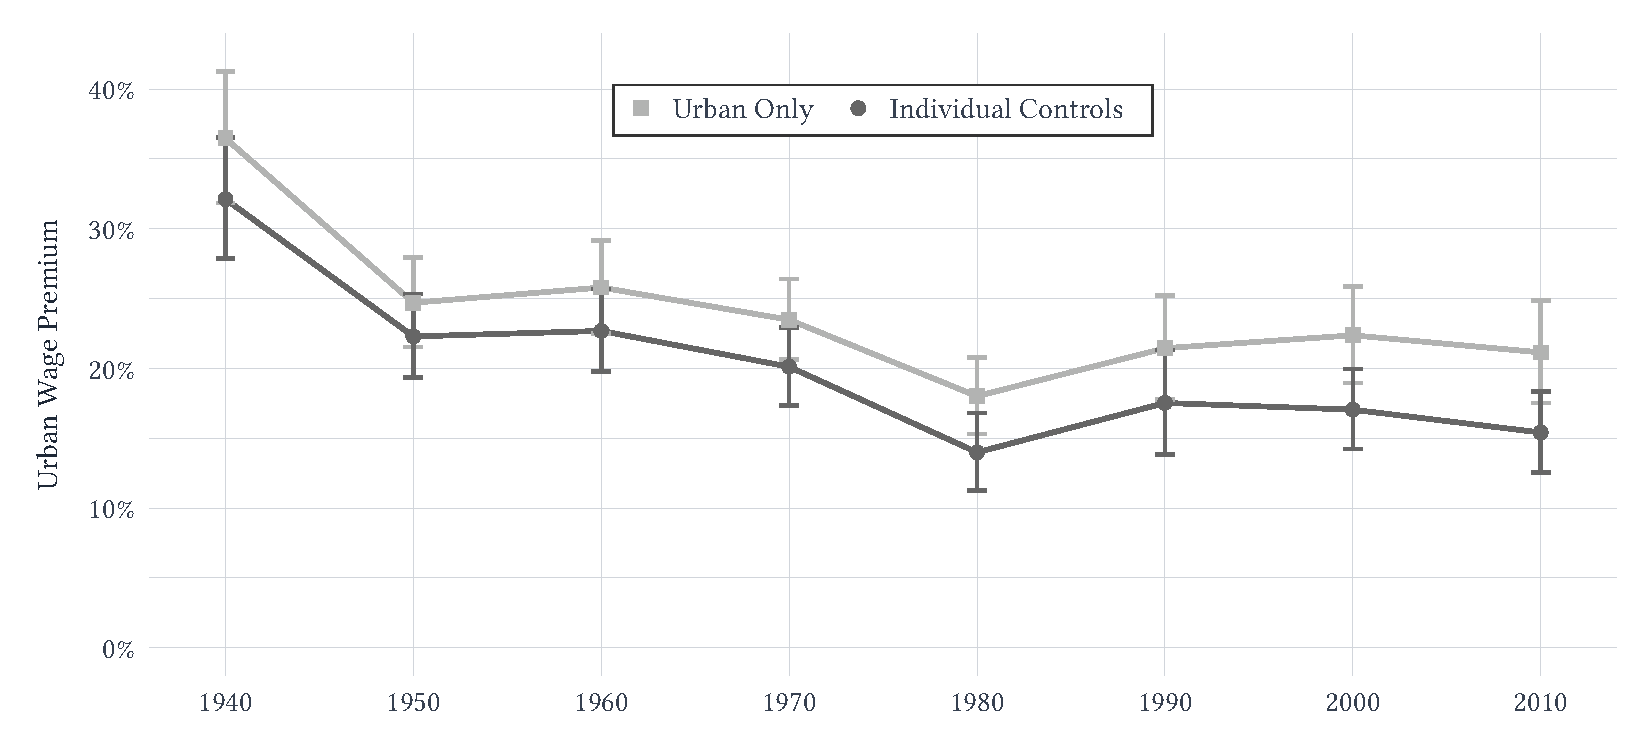
\includegraphics{figures/urban_premium/controls.pdf}
  \end{adjustbox}
  {\footnotesize\singlespacing
      \textit{Notes:} This figure plots the coefficient for survey-year level estimates of the urban wage premium from equation (\ref{eq:controls}) with different level of controls.
      The light gray line with square markers recreates the unadjusted point estimates.
      The dark gray line with circle markers includes controls for age in 5-year bins, education levels, and an indicator for being White.
      The points for each line are plotted with the 95 percent confidence intervals.
  }
\end{figure}
%%%%%%%%%%%%%%%%%%%%%%

The results of estimating equation (\ref{eq:controls}) with and without controls are displayed in Figure \ref{fig:premium_over_time}.
The grey line with square markers reports the mean urban wage difference without any covariates included.
The mean urban differential was highest in 1940 at around 35 percent and falls to a little under 25 percent by 1970.
Starting around 1980, the urban wage difference stabilizes at around 20 percent, where it remains to the present.
The medium grey line with circle markers reports estimates that include individual-level controls in the specification.
Adding individual-level covariates reduces the wage differential in all years.
In 1940, individual characteristics explained roughly 10 percent of the earnings gap between non-urban and urban locations.
By 2010, differences in individual-level observables explained about 25 percent of the gap.
Relative to prior literature such as \citet{Yankow_2006} and \citet{Glaeser_Mare_2001}, our set of observables explains less of the wage differential; however, we are more limited in our set of observable individual-level characteristics. 

Overall, the pattern of wage differentials is similar once individual-level characteristics are included.
We also show that individual characteristics explain a larger share of the urban wage differential over time.
This suggests that sorting -- despite our limited set of observables -- is increasing over time and is consistent with the raw data in Table \ref{tab:summ}.\footnote{
The reason for the difference in estimates relative to \citet{Boustan_Bunten_Hearey_2013} who find a U-shaped pattern comes from our use of a regression framework.
The method in \citet{Boustan_Bunten_Hearey_2013} estimates $ \log( \hat{\mathbb{E}}[\text{Wage} \ |\  \text{Urban} = 1] ) - \log( \hat{\mathbb{E}}[\text{Wage} \ |\  \text{Urban} = 0] )$, which differs from the regression estimate, $\hat{\beta}_1 = \hat{\mathbb{E}}[ \log(\text{Wage}) \ |\  \text{Urban} = 1] - \hat{\mathbb{E}}[ \log(\text{Wage}) \ |\  \text{Urban} = 0]$.
The latter is a more precise estimate for average percent difference in wages.}

%%%%%%%%%%%%%%%%%%%%%%%%%%%%%%%%%%%%%%%%%%%%%%%%%%%%%%%%%%%
\section{Sorting and the Urban Wage Premium}\label{sec:sorting}
%%%%%%%%%%%%%%%%%%%%%%%%%%%%%%%%%%%%%%%%%%%%%%%%%%%%%%%%%%%

In this section, we turn to quantifying the causal urban wage premium by controlling for unobserved characteristics that may drive sorting.
Sorting behaviors by workers can lead the urban indicator to be correlated with the average unobservable differences between urban and non-urban workers.
The urban wage premium estimate therefore is contaminated by the fact that urban workers and non-urban workers have different underlying productivities. 
The urban wage premium literature often uses individual panel data to isolate the effect of living in an urban area by observing individuals who transition across urban and rural locations.\footnote{
  For a recent example that uses matched employee-employer data, see \citet{FRINGS2022103786}.
  Additionally, \citet{eckert2022return} utilizes the placement of refugees in Denmark to estimate the returns to urban experience.
} 
Given the cross-sectional nature of our data, we cannot adopt these panel data methods.

To overcome the empirical challenge of worker's selection into urban locations in cross-sectional data, we use properties of a location choice model to control for sorting as proposed by \citet{altonji2018estimating}. 
The canonical location choice model assumes that willingness to pay for amenities varies based on both observable and unobservable characteristics of the worker.  
This leads workers to sort across locations based on differences in location-specific amenities.
Empirical data clearly show differences in location decisions across individuals with varying observable characteristics \citep[e.g.][]{Diamond_2016}.

At the core of our approach is the following intuition.
One observable characteristic that varies across locations is the percentage of workers with a college degree.
This variation could be driven by differences in consumptive amenities across locations, such as access to cultural activities, restaurants, or recreational spaces.
Workers with different unobserved characteristics (such as varying work ethics and levels of creative intelligence) may also sort based on consumptive amenities.
Hence, the average observable characteristics of workers can provide insights into differences in average unobservable characteristics, even if the precise relationship between them is unknown. 
\citet{altonji2018estimating} show that under the standard location choice model, the mapping from location-level averages of observable variables to averages of unobservable variables is linear, which is crucial for our estimation approach.
We utilize this linear mapping by incorporating group-level averages of observable individual characteristics into our baseline estimating equation to control for sorting on unobservable traits.\footnote{
  In this setting, observable and unobservable characteristics are a function of amenities, and  can be inverted as a function of observed characteristics (i.e., group average observables).
}

More formally, consider an indirect utility function over locations $s$ that is additively separable in amenities ${A}_s$ and prices ${P}_s$: 
\begin{equation} \label{eq:loc choice}
    \text{V}_i(s) = {W}_i{A}_s + \varepsilon_{si} - {P}_s.
\end{equation} 
${W}_i$ represents individuals' underlying willingness to pay for each latent amenity.\footnote{
  This multinomial model of utility is common in urban economics \citep*[e.g.][]{Kline_Moretti_2014,diamond2021spatial}.
}
\citet{altonji2018estimating} then define $\text{W}_i$ as an additive function of observable characteristics ${X}_i$ and unobservable characteristics ${X}_i^\text{U}$. 
Under the assumptions, the utility function can be rewritten as a function of individual-level observables, individual-level unobservables, amenities, and prices:
\begin{equation}\label{eq:loc choice sub}
    \text{V}_i(s) = ({X}_i\Theta + {X}_i^\text{U}\Theta^\text{U}) {A}_s + \varepsilon_{si} - {P}_s.
\end{equation} 
Individuals choose where to live to maximize utility over all locations, taking the amenities, prices, and individual characteristics as given. 

\citet{altonji2018estimating} make five modeling assumptions: First, preferences are given by equation \eqref{eq:loc choice sub}.
Second, $\varepsilon_{si}$ has mean zero and is independent of observables, unobservables, and amenities for all locations.
Third, prices and amenities in each location are viewed as exogenous to the individual when choosing their location.
Importantly, housing prices are allowed to adjust from sorting in the aggregate and our we only assume that individuals do not consider their own effect on the prices when making their decision.
Fourth, the expectation of ${X}_i$ conditional on ${W}_i$ and the conditional expectation of ${X}_i^U$ are both linear in ${W}_i$.  
Fifth, there are at least as many observable characteristics as unobservable characteristics.
The last two conditions require that the set of location-specific factors that drive sorting on \emph{observable} covariates contains \emph{all} location-specific factors that drive sorting based on \emph{unobservable} covariates.\footnote{
  \citet{Diamond_2016} provides evidence using a principal component analysis on a very detailed set of amenities and documents that the effective rank of amenities is around five (with three components explaining most of the variation).
  In the context of this paper, the key identifying assumption is that our group-average variables have an effective (column) rank larger than five.
  Empirically, we run principal components analysis and find more than five components that explain more than 5 percent of the total variance across years.
  This provides support for using the approach in \citet{altonji2018estimating} to address sorting.
} 
The intuition for this approach is that the regression will first ``invert'' the observed group-level averages to location-specific amenities from the fourth assumption above.
Then these amenities can be linearly projected to group averages of the unobservable covariates using the fourth and fifth assumption.
Hence, controlling for group averages of observed characteristics is sufficient to control for the sorting based unobserved characteristics.\footnote{
  The above ``inversion'' is only possible if the mapping between group averages and location-specific amenities is one-to-one.
  If there are more amenities than group-average variables, then a unique inverse will not exist.
  Hence, the rank of observables must be larger than the unobservables.
}

Taking this approach, we rewrite equation (\ref{eq:controls}) to include group-level averages of the individual characteristics in each location.
In particular, we estimate:
\begin{equation}
    \label{eq:AM}
    \log \text{wage}_i = \beta_0 + \beta_1 \text{urban}_i + \bm{X}_{i} \delta + \bar{\bm{X}}_{c(i)}\gamma + \varepsilon_i,
\end{equation} 
where $\bar{\bm{X}}_{c(i)}$ are the location-specific average of the individual characteristics in $\bm{X}_i$ and additional location-invariant characteristics.\footnote{\label{footnote:group_averages}
  We include as group-averages the share of white workers (the share of non-white workers drops out); share of residents in all but one of the age groups; share that are veterans; share that are married and together, married and apart, and single; and share with less than a high school degree, share with a high school degree, share with some college, share with BA degree, and share with advanced education.
  Additionally, we include a measure of market access calculated as in \citet{Jaworski_Kitchens_2019}.
} 
In this case, $\beta_1$ now captures the urban premium after controlling for sorting.
Note that by controlling for the average characteristics of a worker's neighbors, we are, in effect, controlling for peer effects on a worker's wages. 
Our estimate may, therefore, underestimate the true impact of living in a city if it mainly operates through better peer-networks. 
As we will see below, given that we match other estimates found using panel data, this alleviates some concern.
\kyle{Thoughts on this?}


%%%%%%%%%%%%%%%%%%%%%%
\begin{figure}[t]
  \caption{Urban Wage Premium Controlling for Individual Characteristics and Sorting Using Group-Level Averages, 1940-2010}
  \label{fig:causal_premium}
  {\centering
      \resizebox{\columnwidth}{!}{
        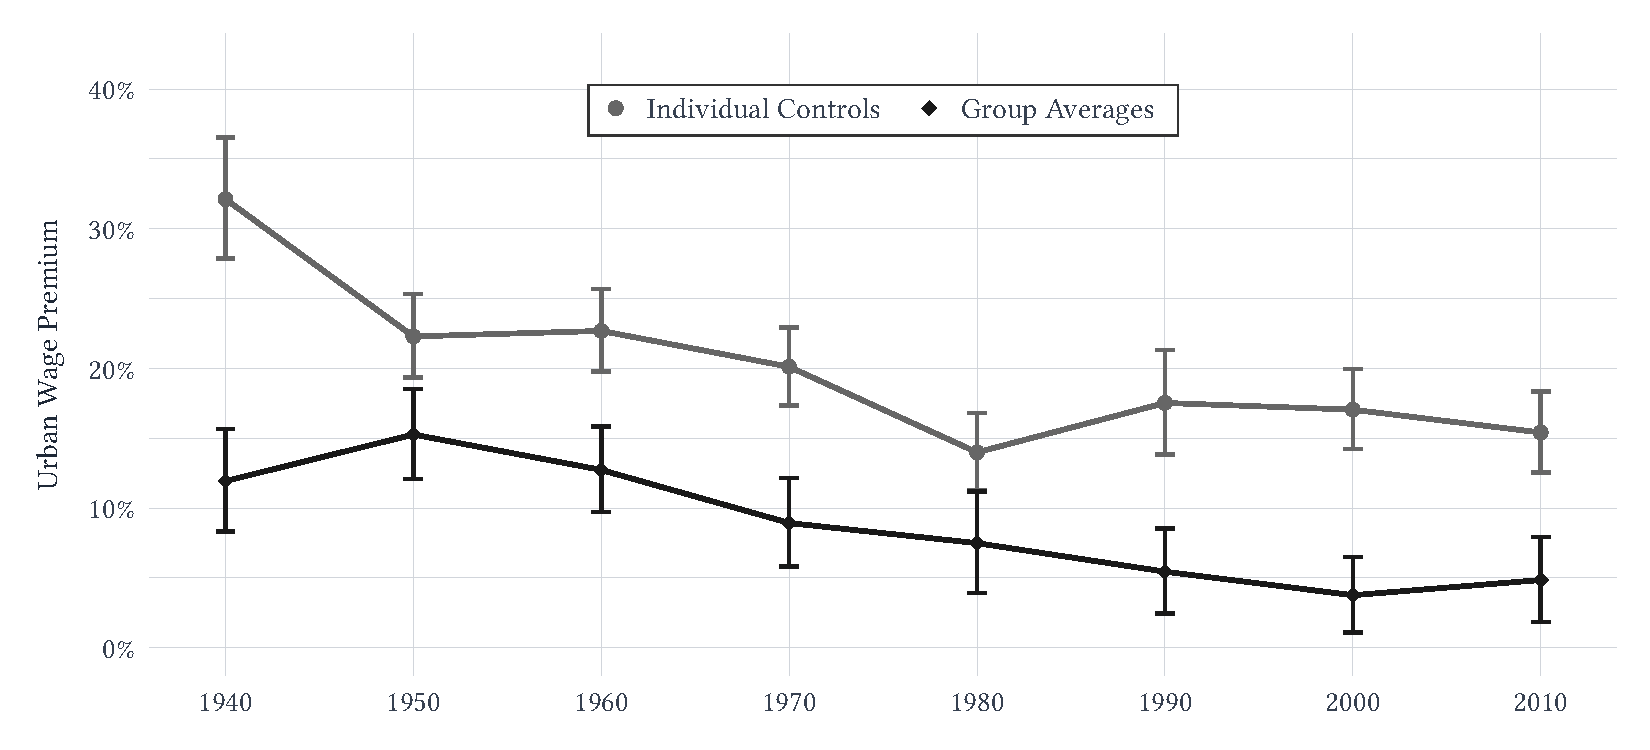
\includegraphics{figures/urban_premium/controls_and_causal.pdf}
      } 
  }%
  {\footnotesize\singlespacing
      \textit{Notes:} This figure plots the coefficient for survey-year level estimates of the urban wage premium following the methodology in Section \ref{sec:sorting}.
We estimate equation \eqref{eq:AM} with the individual-level and group-average controls.
These point estimates serve as our estimate for the causal urban wage premium. 
  }
\end{figure}
%%%%%%%%%%%%%%%%%%%%%%

We present our main estimates of equation \eqref{eq:AM} for each year are plotted in Figure \ref{fig:causal_premium}.
These estimates make clear that using the group-level averages of individual characteristics to control for sorting decreases the urban wage premium significantly.
Relative to the raw urban versus non-urban wage differential, our estimates suggest that individual characteristics and sorting explain approximately 75 percent of the wage differential between urban and non-urban areas after 1980 and approximately half in earlier decades.

Focusing on the period between 1980 and 2010, when our estimates overlap those reported in the existing literature, we find an urban wage premium of approximately 5 percent in each year.
Our estimates closely match those reported in \citet*{Glaeser_Mare_2001}, who report a premium of 4.5 percent in the densest metropolitan areas.
Our estimates also mirror those reported by \cite*{Yankow_2006}, whose fixed effects estimates range from 4.9 to 5.4 percent.
Our estimates are also within the range of those reported in \citet*{BaumSnow_Pavan_2012}.
The overlap of our estimates for the decades since 1980 and previous estimates provides support for our approach using group-level averages to address the potential role of sorting.

Next, we turn to the period from 1940 to 1980, where the previous literature has yet to provide estimates of the urban wage premium.
In 1940, we find that the urban wage premium was approximately 13 percent.
Given a raw differential of 31 percent, sorting and individual characteristics explain about three-fifths of the urban versus non-urban wage gap.
Between 1940 and 1970, we estimate that the urban wage premium fell substantially.
The premium stayed high at 16 percent in 1950 and 13 percent in 1960 and then began to decline to about 5 percent starting in the 1990s.

The estimates for the period from 1940 to 1970 are striking.
Our estimates for the earlier period are more than twice the size of those reported in the literature for the period between 1980 and 2020.
The recent literature has sought to explain the widening urban versus non-urban wage gap since 1970, largely focusing on the differential return to skill in urban areas \citep*{ganong2017has, baum2018has, dauth2018matching, autorWorkPastFuture}.
For example, \citet{baum2018has} and \citet{autorWorkPastFuture} highlight that the returns to education in urban areas increased starting in 2000 due to agglomeration forces that are skill-biased. 

\begin{figure}[t]
  \caption{Urban Wage Premium Using the 1940 Definition of MSAs, 1940-2010}
  \label{fig:premium_msa_in_all_yrs}
  {\centering
    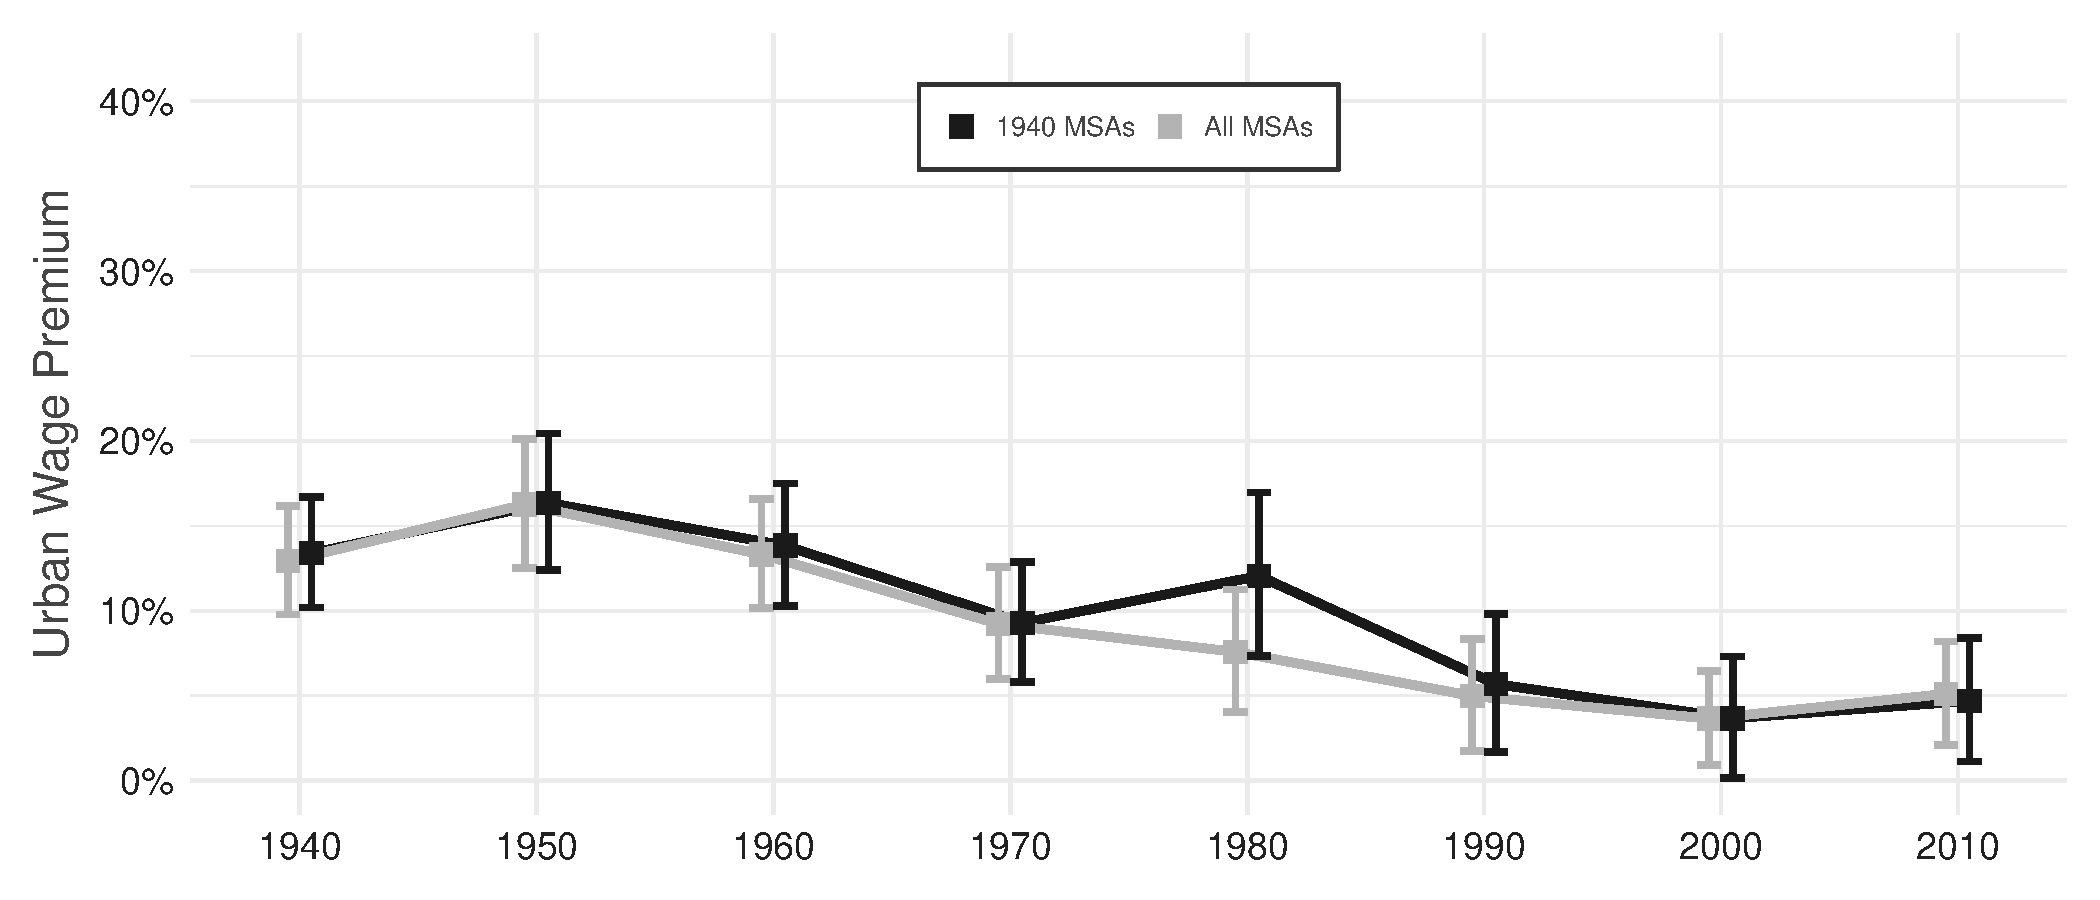
\includegraphics[width=\textwidth]{figures/urban_premium/1940_msas_compared.pdf}
  }

  {\footnotesize\singlespacing
      \textit{Notes:} This figure plots the coefficient for survey-year level estimates of the urban wage premium following the methodology in Section \ref{sec:sorting}.
We estimate equation \eqref{eq:AM} with the individual-level and group-average controls using only the subsample of 1940 MSAs.
Individuals living in MSAs that were added after 1940 are dropped from the sample.
The estimates from Figure \ref{fig:causal_premium} are reproduced for comparison.
  }
\end{figure}

Our estimates suggest that earlier periods of rapid change affected the wage differential between urban and non-urban areas.
We show that sorting became increasingly important in postwar period, which is earlier than previously documented.
Broadly, these results reinforce the focus of \citet{autorWorkPastFuture} and \citet{papageorgiou2022occupational} on the changing number and composition of occupations available for low-skill workers in this period.
For example, our estimates are consistent with the wave of factory automation in the 1950s and early 1960s. 

Over time, the number of MSAs grows as new cities increase in size.
This raises a concern that our estimates may reflect a change in the composition of MSAs.
To rule this out, we re-estimate equation \eqref{eq:AM} with a fixed sample of MSAs based on their 1940 designations and drop observations from MSAs designated after 1940 from the sample.
In Figure \ref{fig:premium_msa_in_all_yrs} we report the estimates holding the set of MSAs constant.
The results are similar to our baseline estimates, suggesting that the changing composition of cities does not bias our estimates.    

\section{Urban Wage Premium Adjusted for Housing Costs}

So far we have ignored the role that rents have in determining an individual's `real wage'.
Canonical urban models suggest that urban rents will adjust in response to higher wages and partially absorb the wage premium, such that utility is equalized across space.  

To ensure that the urban wage premium we estimate is not driven by rent differentials, we re-estimate equation \eqref{eq:AM} using a measure of income that accounts for location-specific differences in housing costs.\footnote{
  For example, between 1960 and 2010, the average rent in an MSA was between 50 and 70 percent higher than non-MSA regions.
}
Following \citet{ganong2017has} and \citet{hoxie2020moving}, we use both rent and home value in calculating the cost of housing. 
For rent, we use the monthly rent and divide it by 4 to get weekly rent.\footnote{
  For 1950, microdata on rent is not available, so instead we use the average rent as reported in census summary tables.
}
For home values, we set the annual housing cost at 5\% of the home value and divide by 48 for weekly costs. 
Then our housing cost is subtracted from the reported weekly wage to get that individual's net-wage.

Figure \ref{fig:raw_net_premium} plots the raw wage premium after subtracting the cost of housing. This figure shows that in the raw data, a portion of the wage premium is extracted by landlords via a higher rent premium. 
Turning to our causal estimates in figure \ref{fig:causal_net_premium}, the results after 1970 do not seem to significantly change. 
However, the estimated wage premium from 1940-1960 shrinks slightly to between 5 and 10\%. 
These results suggest that some of the causal benefits of cities that accrued to worker was lost to higher rents between 1940 and 1960.

%%%%%%%%%%%%%%%%%%%%%%
\begin{figure}[t!]
  \caption{Urban Wage Premium Net of Housing Costs, 1940-2010}
  \begin{subfigure}{\linewidth}
    \caption{Raw Differences}
    \label{fig:raw_net_premium}
    \begin{adjustbox}{width=\textwidth,center}
      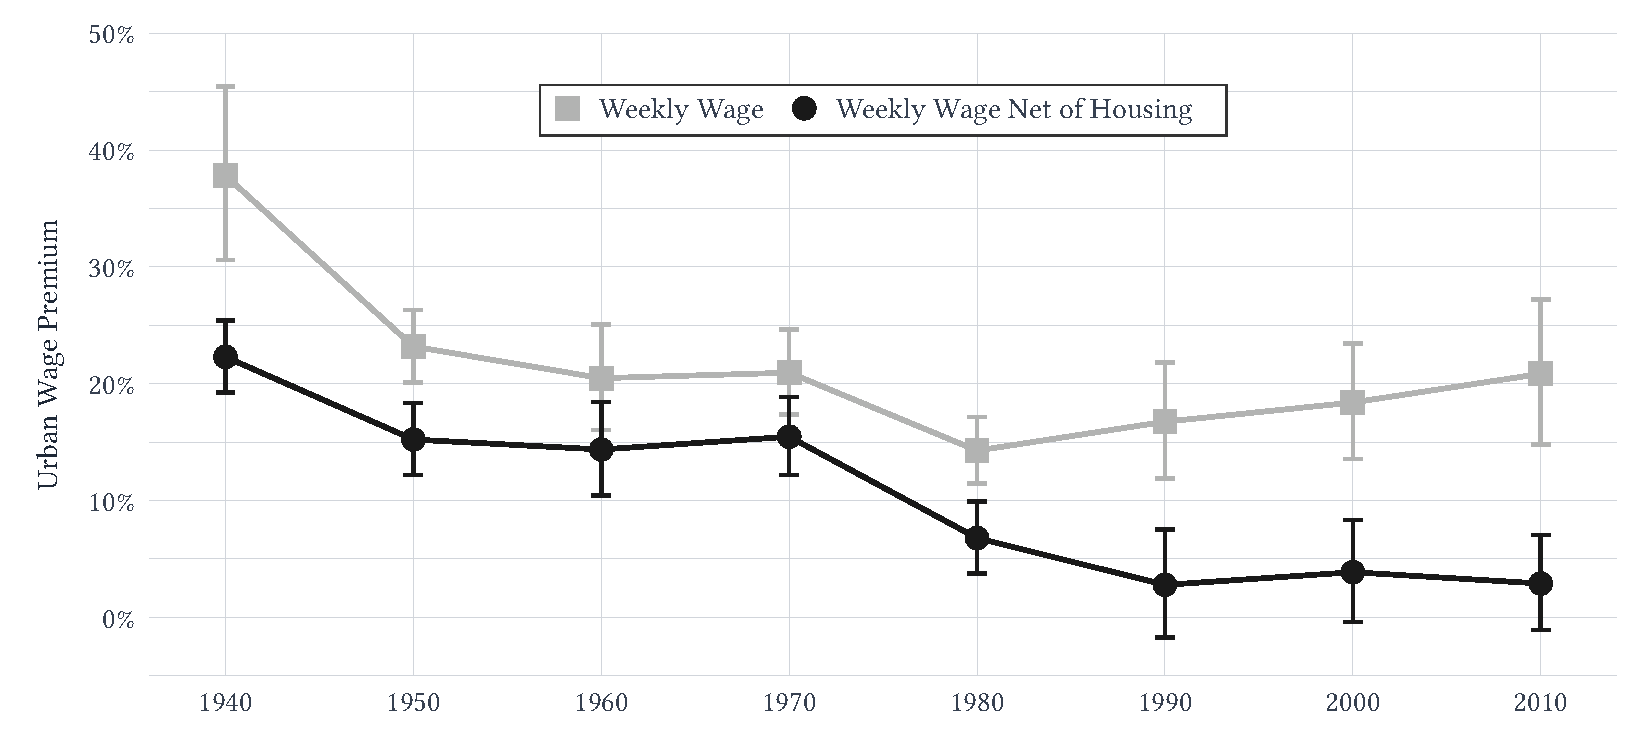
\includegraphics{figures/housing_costs/net_raw.pdf}
    \end{adjustbox}
  \end{subfigure}
  \begin{subfigure}{\linewidth}
    \caption{Controlling for Individual Characteristics and Sorting Using Group-Level Averages}
    \label{fig:causal_net_premium}
    \begin{adjustbox}{width=\textwidth,center}
      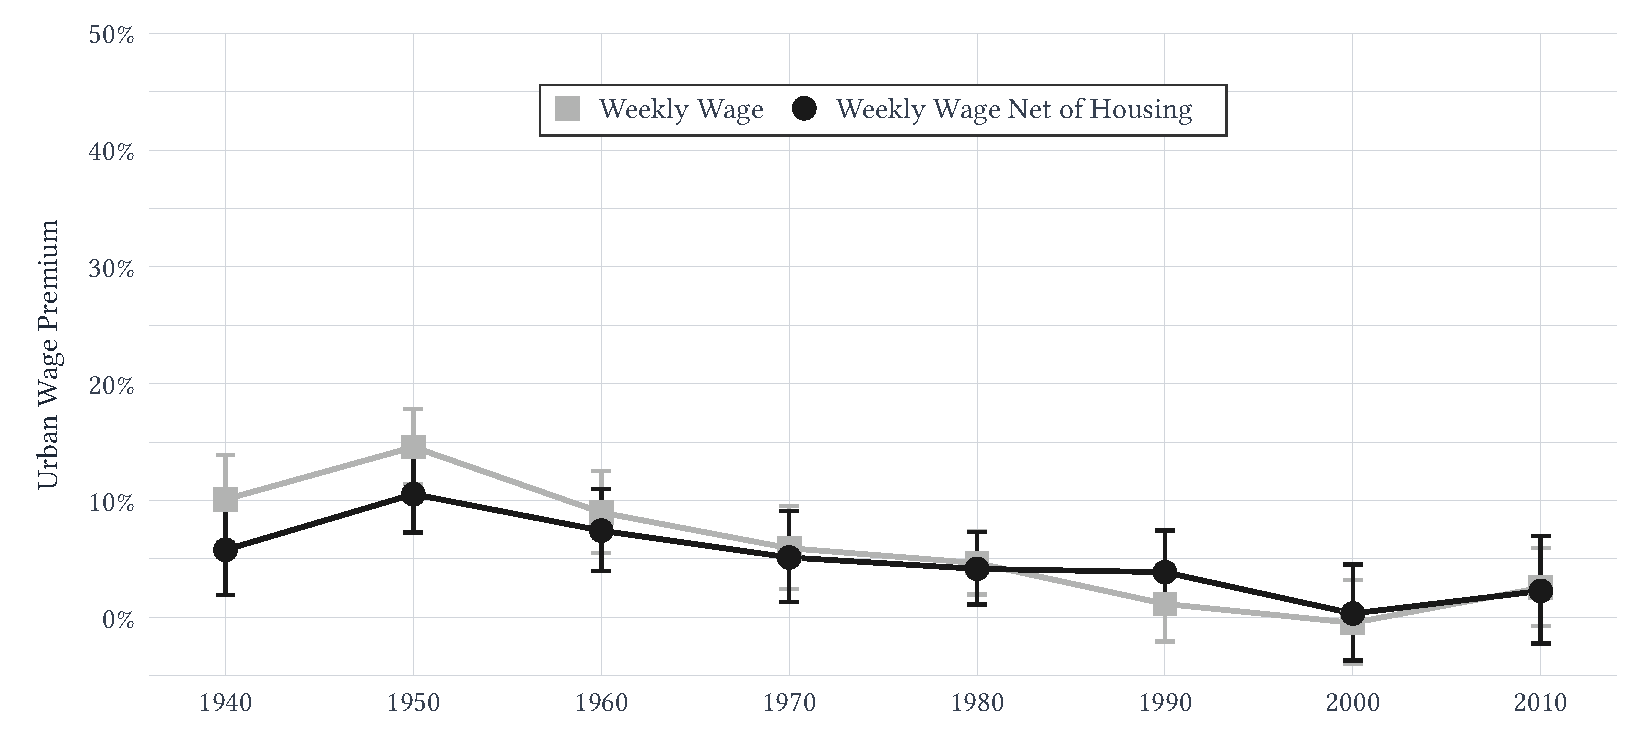
\includegraphics{figures/housing_costs/net_causal.pdf}
    \end{adjustbox}
  \end{subfigure}

  {\footnotesize\singlespacing
    \textit{Notes:} This figure recreates figures \ref{fig:premium_over_time} and \ref{fig:causal_premium} using a modified wage measure that subtracts off the cost of housing. 
  }
\end{figure}
%%%%%%%%%%%%%%%%%%%%%%



\section{Heterogeneity by City Size, Region, and Indvidiaul Characteristics}

Up to this point, we have documented the increasing role of sorting in explaining the difference between urban and non-urban wages over time.
Importantly, this pattern may differ substantially throughout the city-size distribution, across regions, or for workers of different characteristics.
In this section, we examine the role of these factors.

Recent literature highlights that the urban wage premium is increasing in city size \citep[e.g.][]{BaumSnow_Pavan_2012}.
To test for heterogeneity in the urban wage premium throughout the city-size distribution, we re-estimate equation \eqref{eq:AM} but allow cities in the 20 most populated MSAs as of 1940 to have a different urban wage premium.
Panel A of Figure \ref{fig:heterogeneity} plots the estimated urban wage premium for the twenty largest MSAs (square markers) versus the remaining MSAs (round markers).
First, we document that the urban wage premium is higher in the largest 20 MSAs relative to smaller MSAs in all years, consistent with the existing literature.
While the largest MSAs generate larger wage premia, the returns to the largest MSAs have declined relative to smaller MSAs in the last 30 years. 

\begin{figure}[b]
  \caption{Heterogeneity of the Urban Wage Premium, 1940-2010}\label{fig:heterogeneity}

  \vspace{2.5mm}
  \begin{subfigure}{\linewidth}
    \caption{By Twenty Largest versus Other Cities}
    {\centering
      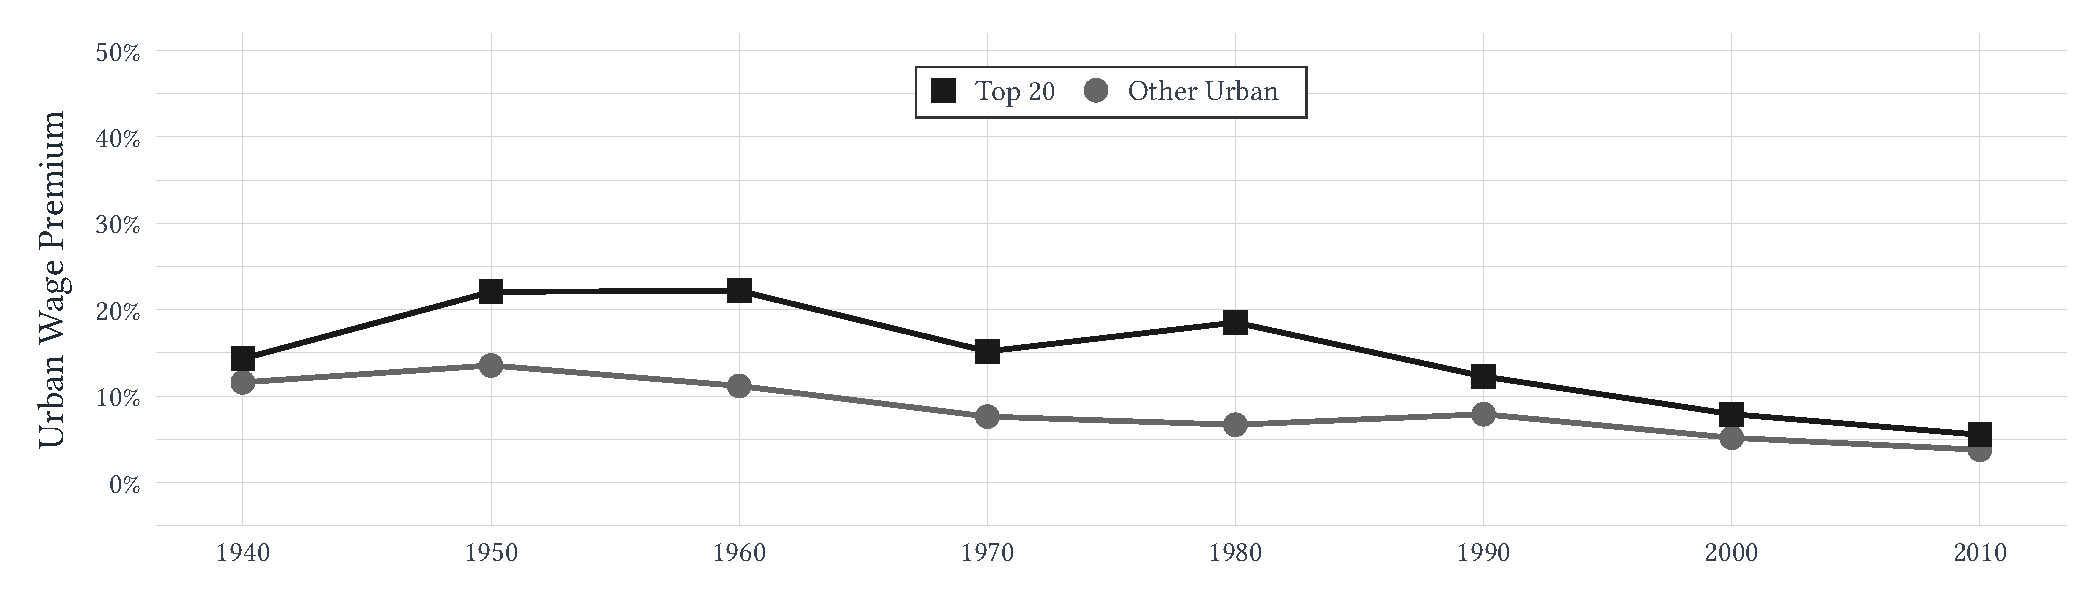
\includegraphics[width=\textwidth]{figures/heterogeneity/by_top20.pdf}
    }
  \end{subfigure}

  \begin{subfigure}{\linewidth}
    \caption{By Census Regions}
    {\centering
      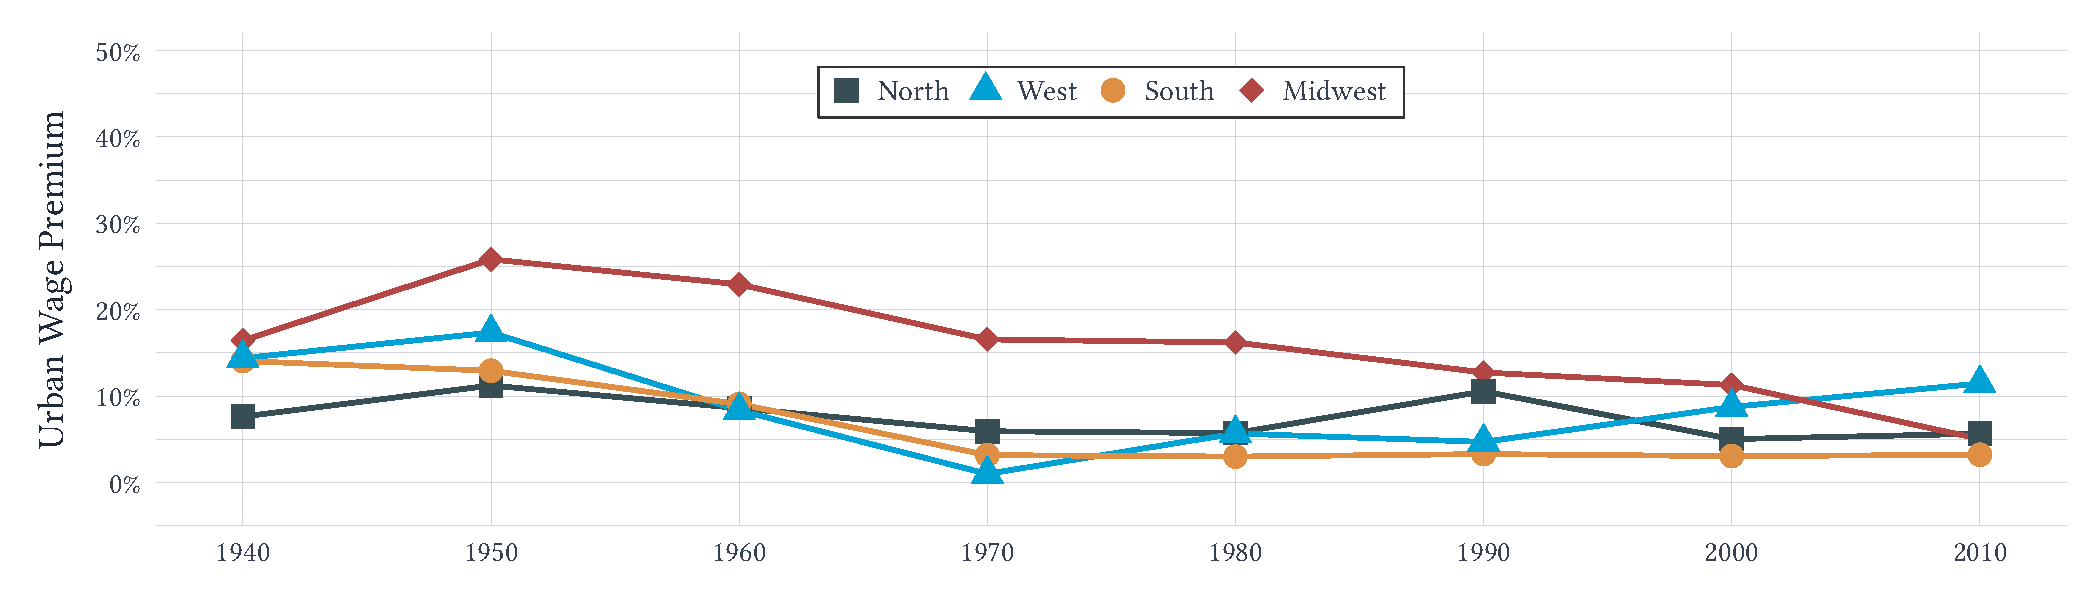
\includegraphics[width=\textwidth]{figures/heterogeneity/by_region.pdf}
    }
  \end{subfigure}
\end{figure}

\begin{figure}[t]\ContinuedFloat
  \begin{subfigure}{\linewidth}
    \caption{College and Non-college Educated Workers}
    {\centering
      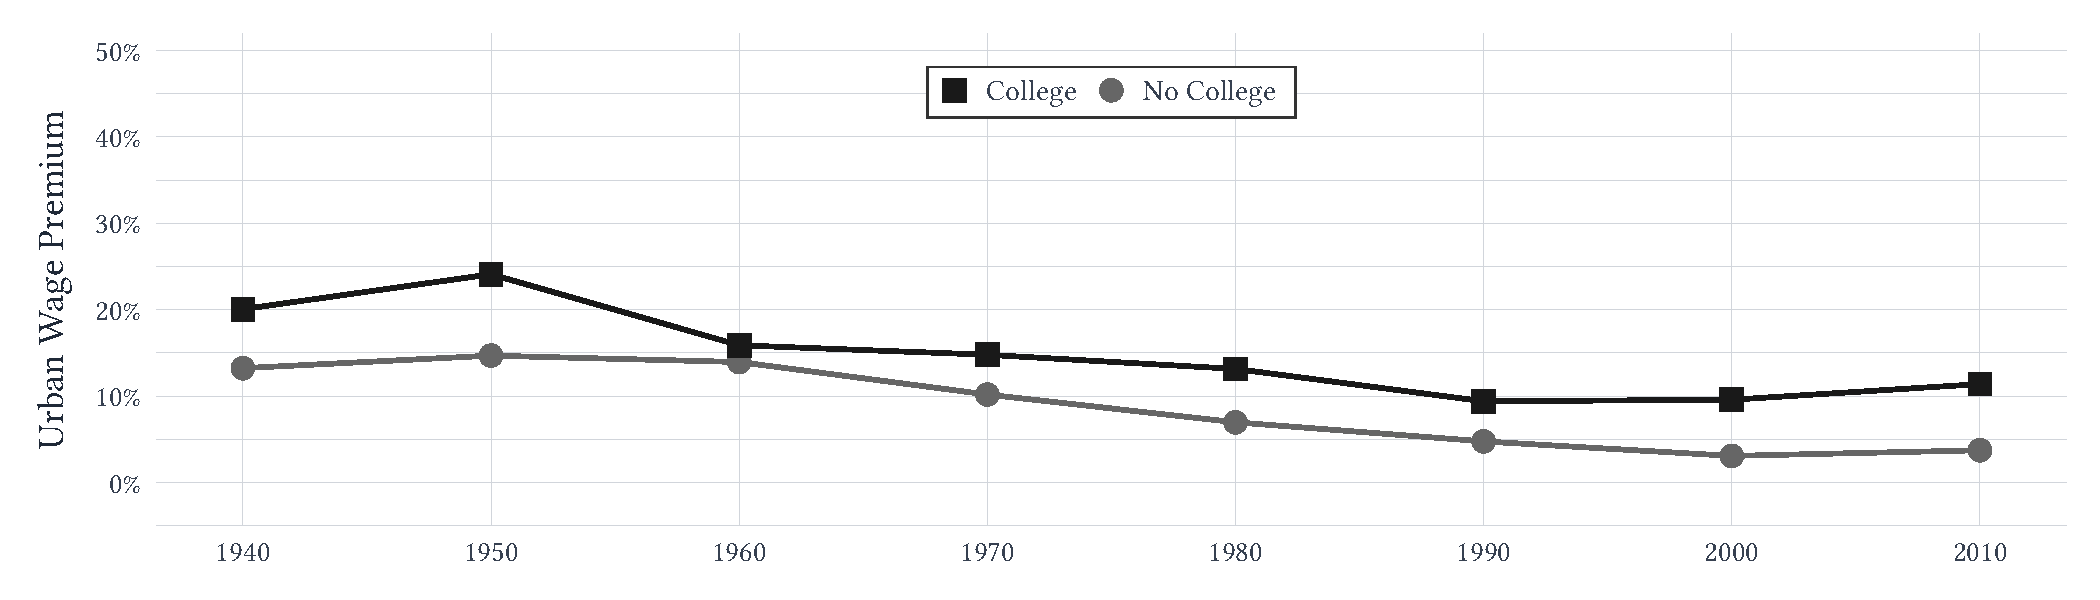
\includegraphics[width=\textwidth]{figures/heterogeneity/by_college.pdf}
    }
  \end{subfigure}

  \begin{subfigure}{\linewidth}
    \caption{White and Black Workers}
    {\centering
      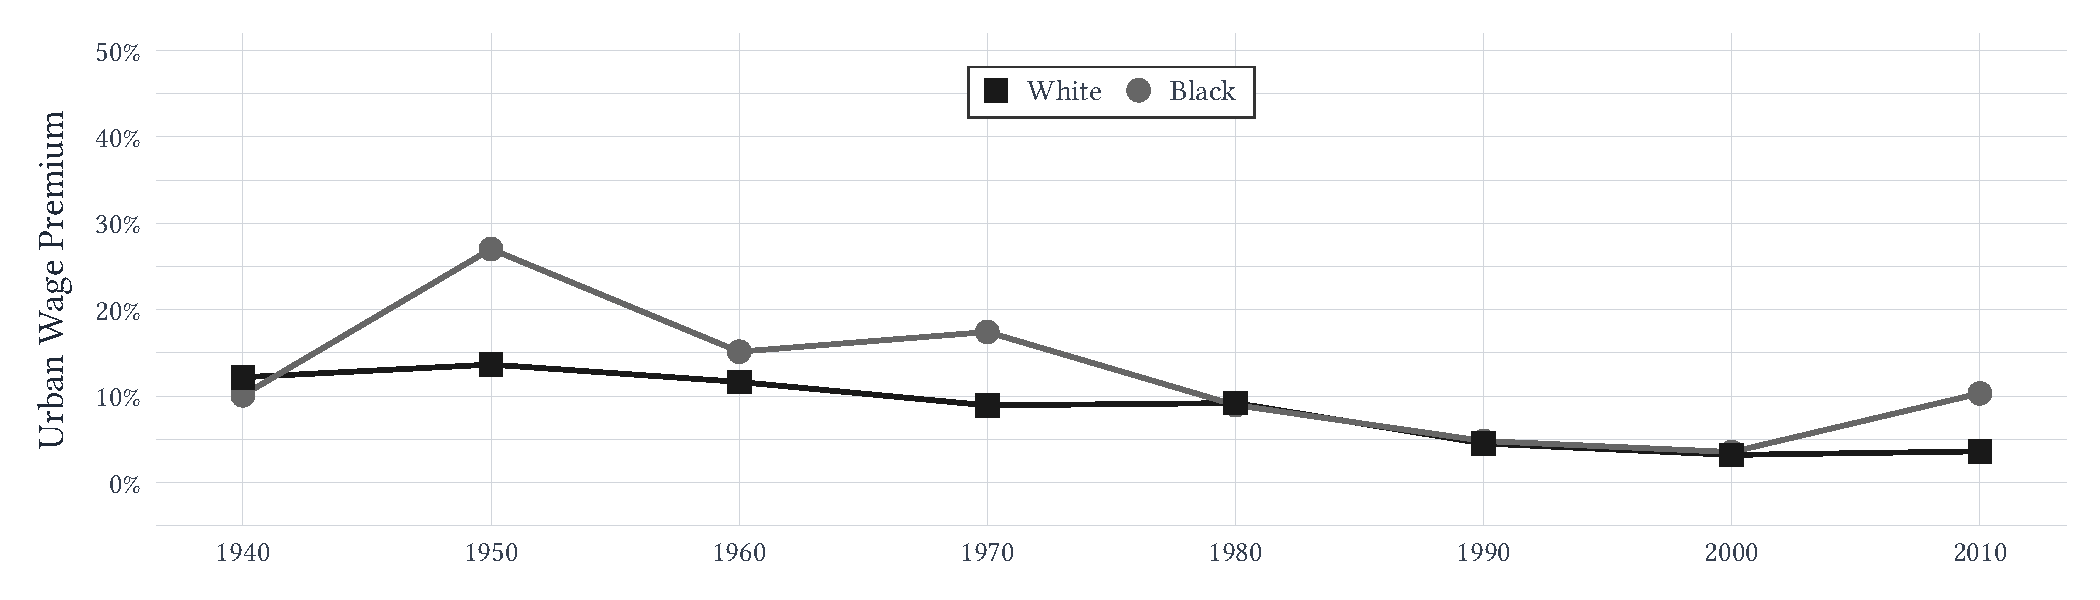
\includegraphics[width=\textwidth]{figures/heterogeneity/by_race.pdf}
    }
  \end{subfigure}

  \begin{subfigure}{\linewidth}
    \caption{Older and Younger Workers}
    {\centering
      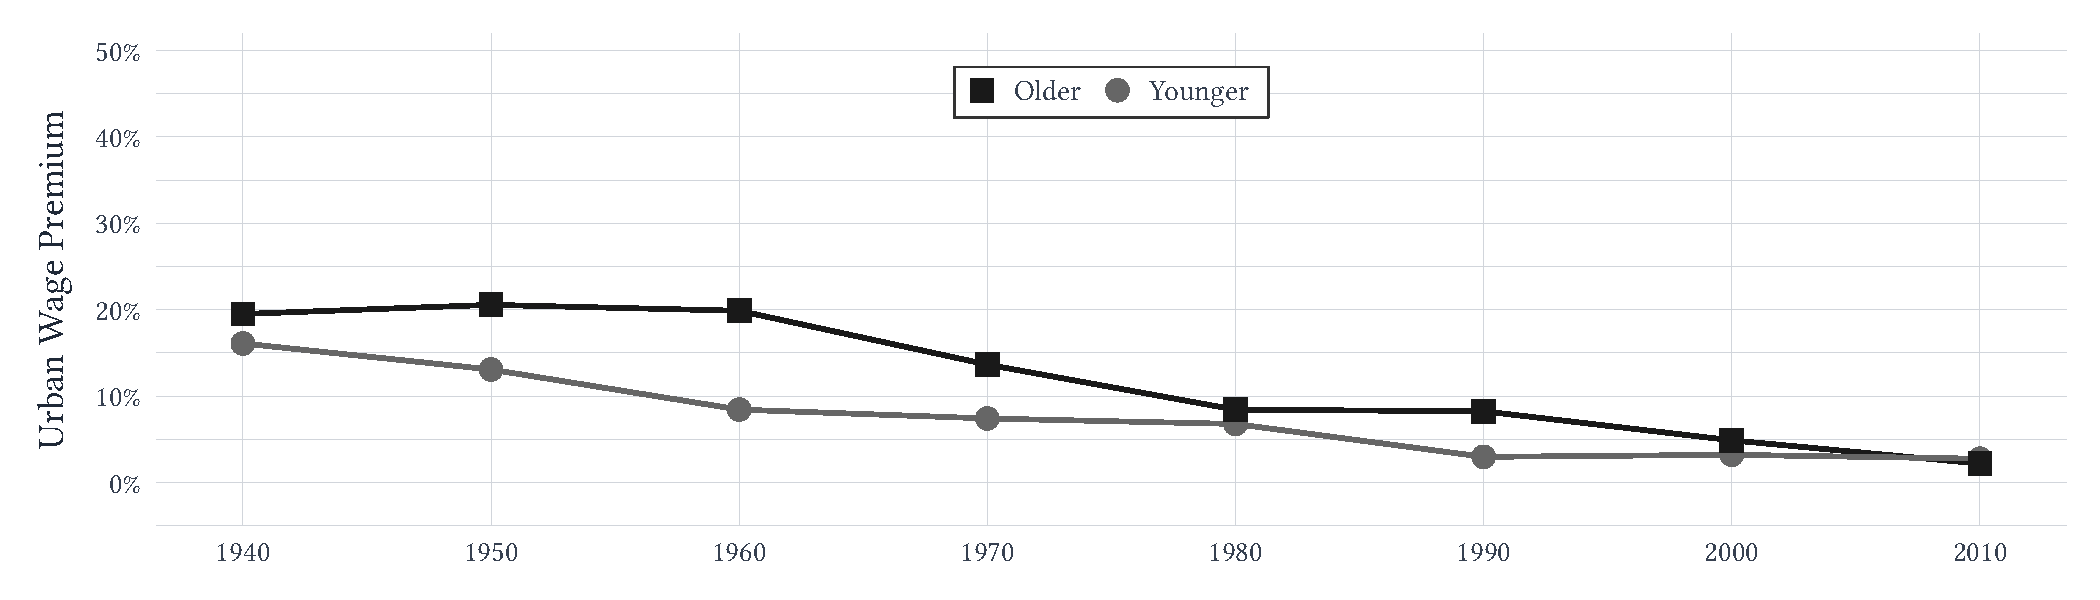
\includegraphics[width=\textwidth]{figures/heterogeneity/by_older.pdf}
    }
  \end{subfigure}
  
  \vspace{-5mm}
  {\footnotesize\singlespacing
      \textit{Notes:} This figure plots the coefficient for survey-year level estimates of the urban wage premium from equation (\ref{eq:controls}) including the individual-level and group-average controls described in footnote \ref{footnote:group_averages} while interacting the urban indicator with three different variables.
      Panel A interacts the urban indicator with an indicator for the top 20 most populous MSA in 1940.
      Panel B interacts the urban indicator with indicators for each census region.
      Panel C reports estimates of equation (\ref{eq:controls}) run on separate samples of college-educated and non-college-educated workers with the group-averages taken separately by sample. 
  }
\end{figure}

Previously, we highlighted how the geography of the highest-wage cities has varied over time.
In the 1940s, the largest premiums were in Rust Belt cities such as Flint, MI and Rochester, NY.
Today, the pattern has shifted towards Sunbelt cities and technology hubs.
Given the shift in the location of work, the relative importance of sorting and agglomeration may also differ across space over the last 80 years.
To explore how the relative importance of sorting varies across geography, we estimate specifications to allow for differences in each census region (i.e., Northeast, South, Midwest, and West).
Panel B of Figure \ref{fig:heterogeneity} plots the estimates.
The Midwest has experienced a large decline in the share of the premium attributable to agglomeration, while agglomeration forces have become relatively more important in the West since 1970. 

As automation and technology have increasingly entered the workplace, the returns to cities may also vary over time for workers with different levels of education.
For example, \citet{gould2007cities} shows that the urban wage premium is significantly larger for white-collar workers.
To explore how agglomeration forces have varied by education group, we estimate separate specifications for college-educated workers and those with less than a college degree.\footnote{
For panels C, D, and E of Figure \ref{fig:heterogeneity}, we calculate the group averages separately by group since we may think that sorting patterns can differ systematically.} 
Panel C of Figure \ref{fig:heterogeneity} plots our estimates by college degree status.
Throughout the period, we generally estimate larger wage premia for college-educated workers, on the order of magnitude of 3-5 percentage points.
Comparing our estimates to \citet{gould2007cities}, we similarly find a premium of around 10 percent for college-educated workers in the 1980s. 

\kyle{I think we need to discuss group-specific averages}
We run \ref{eq:controls} while interacting the urban dummy with a dummy for being a White worker and a dummy for being a Black worker. 
This estimates a race-specific urban wage premium. 
Panel C of Figure \ref{fig:heterogeneity} shows the results. 
Throughout the panel, the Black urban wage premium is estimated to be no smaller than the White premium and in most of the years a larger. 
The Black urban wage premium is estimated to be ten percentage points larger in the middle of the 20th century which is in line with the timing of the Great Migration \citep{derenoncourt2022can}.

Last, \citet{BaumSnow_Pavan_2012} document the urban \emph{wage growth} premium which shows that cities benefit workers by faster wage growth. 
Since we do not have panel data, we can not observe wage growth. 
Instead, we run \ref{eq:controls} separately for indvidiauls in above-median and below-median aged workers\footnote{
  The median age is around 40 across years.
} 
The idea being that older workers have more \emph{potential} time in city and therefore older workers that live in urban areas likely have more cummulative urban experience than younger workers and hence should have a larger premium. 
This hypothesis is borne out by Panel E of Figure \ref{fig:heterogeneity}. An alternative explanation is that the benefits of urban living change over the workers' earning profile. 


\subsection{Distributional Estimates}

In the period after World War II, there were substantial changes in wage inequality. \citet{goldin1992great} discuss the narrowing of the wage distribution in what they label the ``Great Compression'' between 1940 and 1960.
They highlight the rapid increase in the supply increase of educated workers during a period of relatively stagnant demand growth.
Recently, \citet{vickers2021effects} discuss the role of the National War Labor Board on wages in various regions throughout the country and show that wage-setting policies had a meaningful impact on local wage distributions. 

\begin{figure}
  \caption{Distribution of Wage Residuals, 1940-2020}
  \label{fig:9010}

  \vspace{5mm}
  \begin{subfigure}{\linewidth}
    \caption{Aggregate Distribution}
    {\centering
      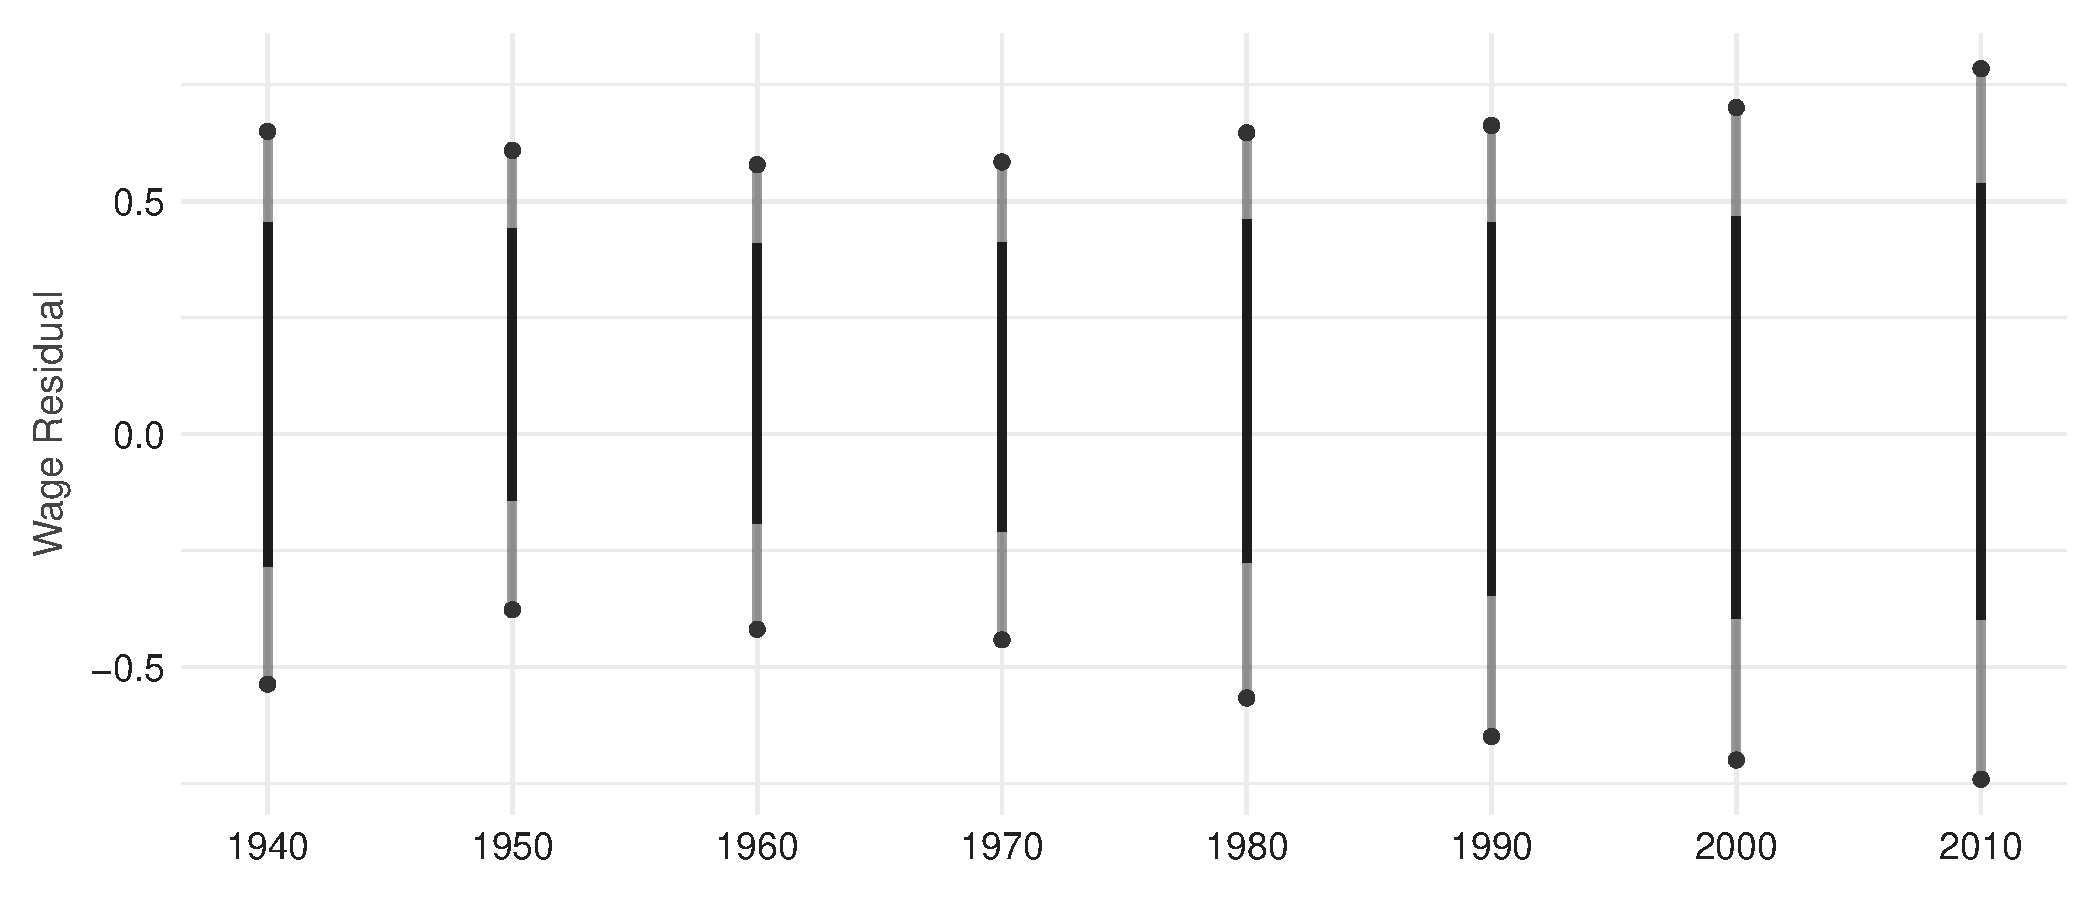
\includegraphics[width=\linewidth]{figures/distribution/9010.pdf}
    }
  \end{subfigure}

  \begin{subfigure}{\linewidth}
    \caption{Urban versus Non-urban Distribution}
    {\centering
      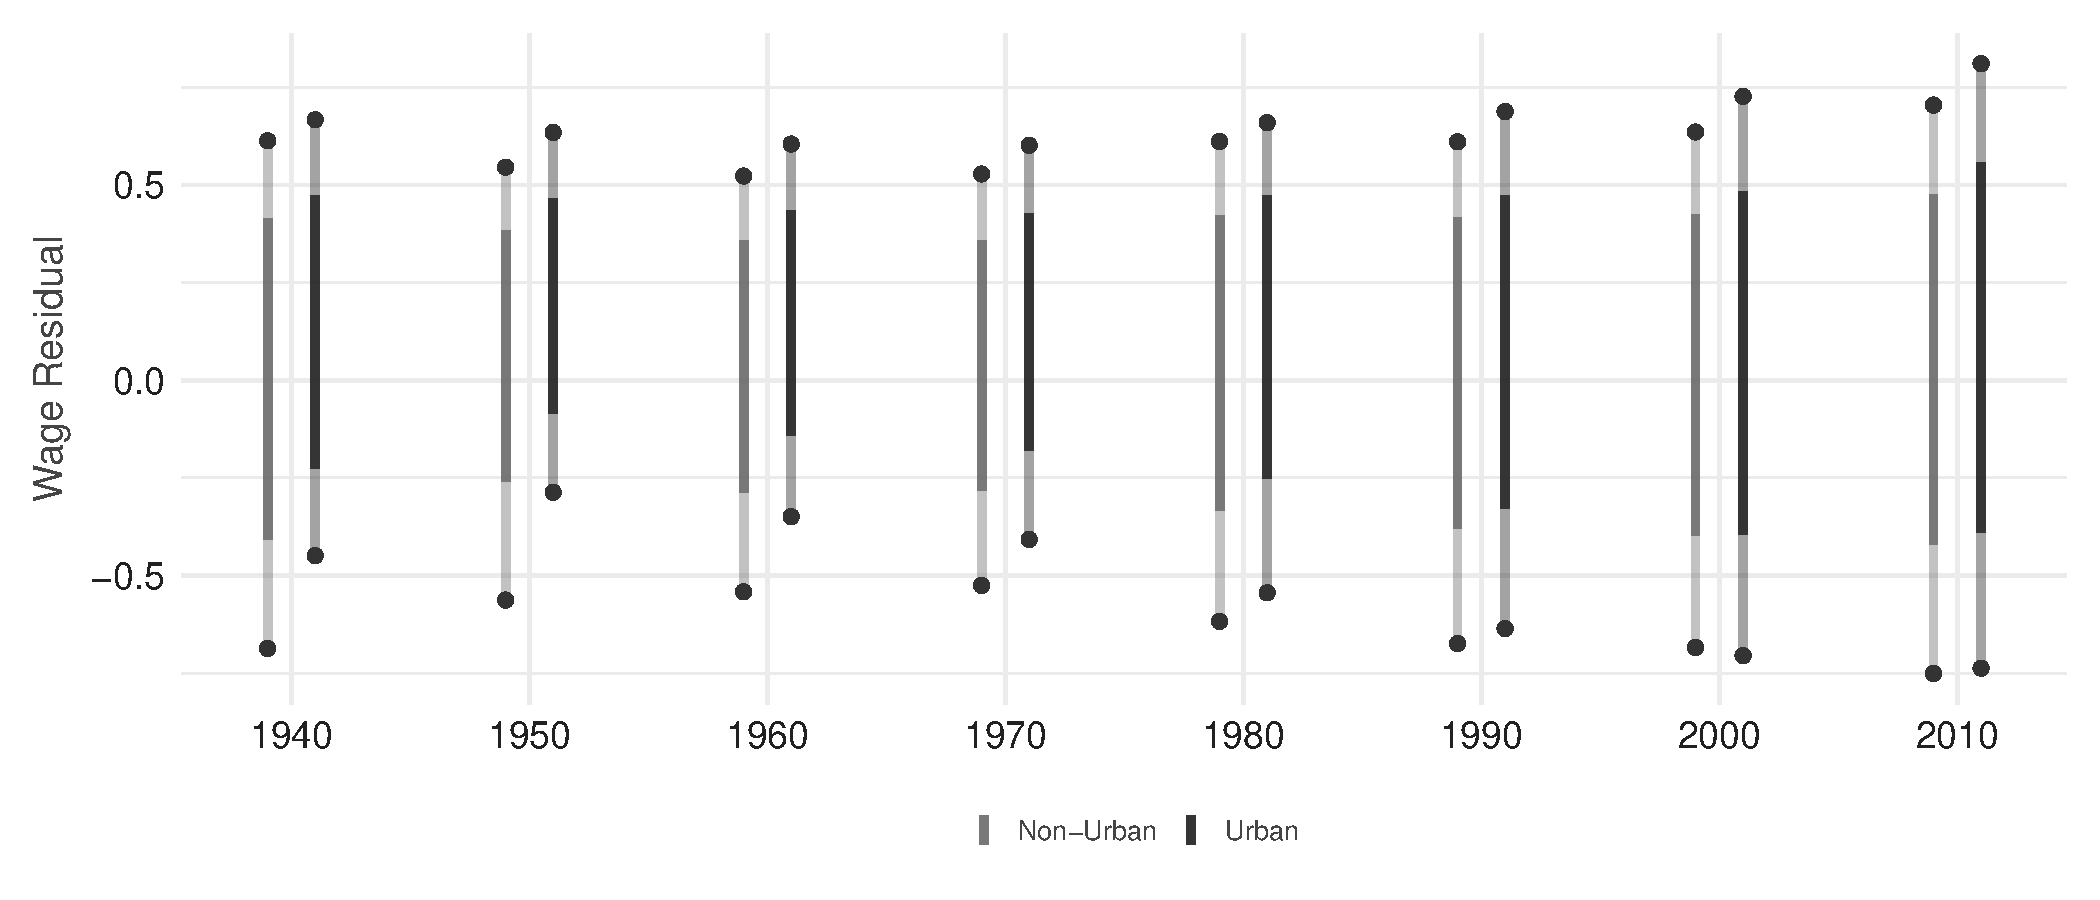
\includegraphics[width=\linewidth]{figures/distribution/9010_urban.pdf}
    }
  \end{subfigure}

  \vspace{-7.5mm}
  {\footnotesize\singlespacing
      \textit{Notes:} This figure takes the residual of wages after regressing on the full-specification and adds back in the causal urban wage premium.
Each panel plots points for the 90th-10th percentiles of the wage residuals and shades darker the 80th-20th percentiles.
Panel A does this for the entire distribution of wages following \citet{goldin1992great}.
Panel B does this separately for urban and non-urban workers.
  }
\end{figure}

To explore whether we observe a compression and then widening of the wage distribution in our setting, we take the residuals from \eqref{eq:AM} which reflect individual earnings after controlling for sorting.
The ninetieth-tenth percentiles summarize the distribution of the wage residuals for each decade in Panel A of Figure \ref{fig:9010}.
Similar to \citet{goldin1992great}, we find evidence consistent with a narrowing of the wage distribution through 1960.
Afterward, the wage distribution widens considerably through 2010.

In Panel B of Figure \ref{fig:9010}, we plot the distribution of residuals for urban and non-urban workers.
In 1940, urban and non-urban workers had a large left tail in the wage distribution, reflecting many workers who earned very low (residualized) weekly earnings.
Between 1940 and 1960 this left-tail disappeared, which provides some evidence that a rising floor potentially drove the Great Compression on non-urban wages.\footnote{
The overall compression and the narrowing of the left-tail are also apparent when using $95^{th}$ and $5^{th}$ percentiles.} \citet{goldin1992great} find similar evidence that increases in the distribution for low-wage workers drove the Great Compression.
Our estimates suggest that the narrowing of the wage distribution occurred in urban and non-urban areas.

%%%%%%%%%%%%%%%%%%%%%%%%%%%%%%%%%%%%%%%%%%%%%%%%%%%%%%%%%%%
\section{Conclusion}
%%%%%%%%%%%%%%%%%%%%%%%%%%%%%%%%%%%%%%%%%%%%%%%%%%%%%%%%%%%


Wages in cities are much higher than in non-urban areas.
Understanding why this gap exists and, in particular, the relative role of sorting versus agglomeration over time is an important topic in urban economics.
In this paper, we quantify the urban wage premium in each decade between 1940 to 2010.
Importantly, we show how to apply the methodology of \citet{altonji2018estimating}, which enables us to use data from annual cross-sections to account for sorting between urban and non-urban locations.
Thus, we provide new estimates of the urban wage premium for the period from 1940 to 1980, while generating estimates for the period from 1980 to 2010 that are similar to those in the existing literature. 

Our results highlight the increasing relative importance of sorting over the second half of the twentieth century and into the first part of the twenty-first century.
By 2010, the relative strength of agglomeration forces was less than half of the agglomeration forces we estimate in 1940.
In addition, we find that this pattern is not driven by changes in the composition of cities in our sample over time or differences in housing costs across cities.
We also show that changes in the urban wage premium and the role of sorting are not due to changes in the returns to city size, regions, level of education, or the structure of the wage distribution across urban and non-urban areas.
Overall, our findings are consistent with a greater role for consumer amenities in explaining the demand for urban living as of 2010.

\clearpage

\setlength{\bibsep}{.01in}
\bibliographystyle{aernobold}
\begin{onehalfspacing}
\bibliography{urban_wage_biblio.bib}
\end{onehalfspacing}

%%%%%%%%%%%%%%%%%%%%%%%%%%%%%%%%%%%%%%%%%%%%%%%%%%%%%%%%%%%

% ------------------------------------------------------------------------------
\appendix 
\numberwithin{equation}{section}
\numberwithin{figure}{section}
\numberwithin{table}{section}
\renewcommand{\thefigure}{\arabic{figure}}
\renewcommand{\thetable}{\arabic{table}}
%\renewcommand{\thefigure}{\Alph{section}\arabic{figure}}
%\renewcommand{\thetable}{\Alph{section}\arabic{table}}

% ------------------------------------------------------------------------------

\newpage\clearpage

\begin{table}[!p]
  \caption{Urban Wage Premium, 1940-2010}
  \label{tab:wage_premium}
  \renewcommand{\arraystretch}{1.25}

  \resizebox{\columnwidth}{!}{
  \begin{threeparttable}
    \begin{tabular}{@{} l *{8}{c} @{}}
      % Head
      \toprule

      & \multicolumn{8}{c}{$\log(\text{Weekly Wage})$}\\
      \cmidrule{2-9}
      
      & 1940 & 1950 & 1960 & 1970 & 1980 & 1990 & 2000 & 2010 \\
        

      % Body
      \toprule
      
\multicolumn{9}{l}{\hspace{-2.5mm}{\bfseries \itshape Panel A: Raw Wage Premium}} \\
$\text{Urban} = 1$ & 0.3162$^{***}$ & 0.2208$^{***}$ & 0.2288$^{***}$ & 0.2109$^{***}$ & 0.1692$^{***}$ & 0.1939$^{***}$ & 0.2014$^{***}$ & 0.1898$^{***}$\\
& (0.0192) & (0.0131) & (0.0134) & (0.0119) & (0.0110) & (0.0158) & (0.0144) & (0.0155)\\
\midrule

\multicolumn{9}{l}{\hspace{-2.5mm}{\bfseries \itshape Panel B: Individual Controls}} \\
$\text{Urban} = 1$ & 0.2822$^{***}$ & 0.2012$^{***}$ & 0.2038$^{***}$ & 0.1833$^{***}$ & 0.1334$^{***}$ & 0.1609$^{***}$ & 0.1566$^{***}$ & 0.1414$^{***}$\\
& (0.0186) & (0.0125) & (0.0123) & (0.0119) & (0.0116) & (0.0163) & (0.0125) & (0.0127)\\
\midrule

\multicolumn{9}{l}{\hspace{-2.5mm}{\bfseries \itshape Panel C: Individual Controls \& Group Averages}} \\
$\text{Urban} = 1$ & 0.1216$^{***}$ & 0.1506$^{***}$ & 0.1251$^{***}$ & 0.0883$^{***}$ & 0.0731$^{***}$ & 0.0487$^{***}$ & 0.0359$^{***}$ & 0.0499$^{***}$\\
& (0.0144) & (0.0167) & (0.0144) & (0.0154) & (0.0171) & (0.0160) & (0.0137) & (0.0147)\\
\midrule

Observations & 2,504,957 & 68,457 & 1,364,524 & 280,338 & 1,907,943 & 2,260,990 & 2,582,144 & 2,718,970\\

      \bottomrule
    \end{tabular}
        
    % Notes 
    \begin{tablenotes}[flushleft]\footnotesize
        \item\textit{Notes.} This table reports coefficient for survey-year level estimates of the urban wage premium from equation (\ref{eq:controls}) with three different level of controls.
The first section includes no controls and represents the urban wage premium observed in the data.
The second section includes controls for age in 5-year bins, education levels, and an indicator for being White.
The final section includes group-average variables following the methodology in Section \ref{sec:sorting}.
These point estimates serve as our estimate for the causal urban wage premium.
        
        \item Signif.
Codes: $^{***}$: 0.01, $^{**}$: 0.05, $^{*}$: 0.1.
Standard errors are clustered  by MSA/CBSA.
    \end{tablenotes}
  \end{threeparttable}
  }

\end{table}

\newpage\clearpage



%\begin{figure}
%  \caption{The Urban Rent Premium, 1940-2010}
%  \label{fig:premium_over_time}
%  {\centering
%      \resizebox{\columnwidth}{!}{
%          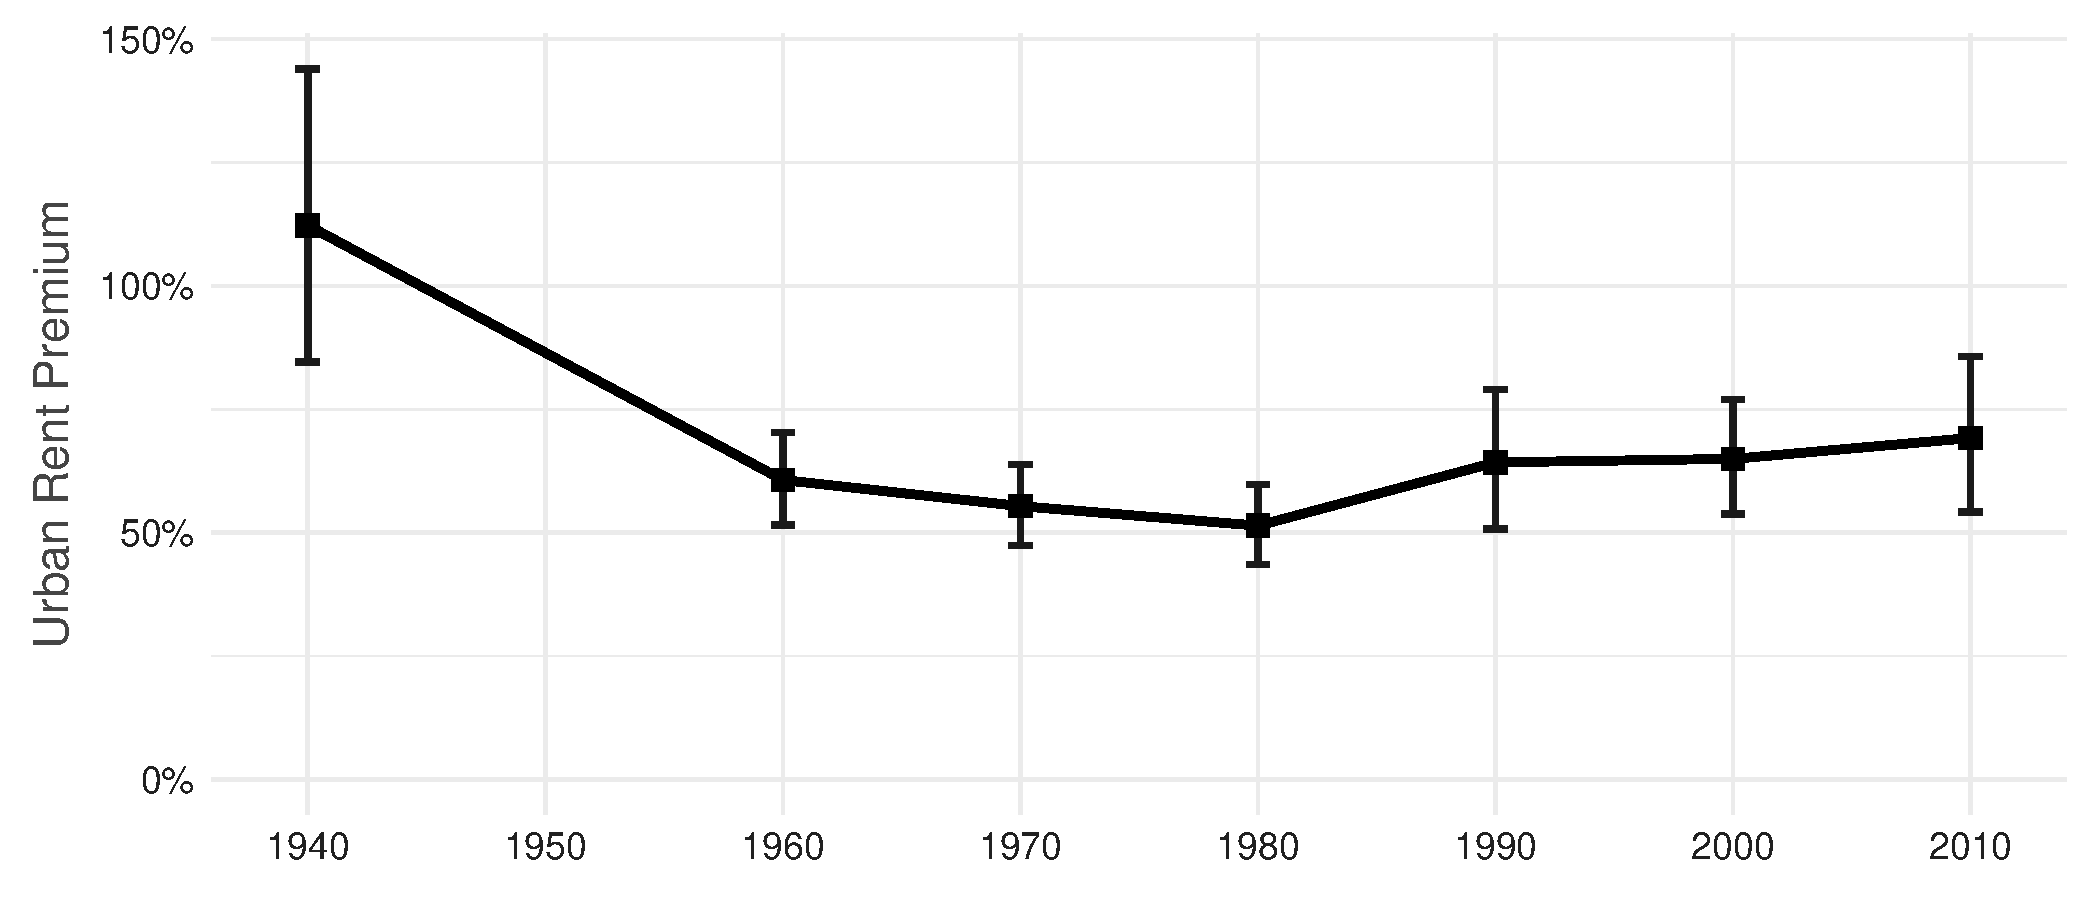
\includegraphics{figures/rentpremium_urban.pdf}
%      } 
%  }%
%  {\footnotesize\singlespacing
%      \textit{Notes:} This figure plots the coefficient for survey-year level estimates of the urban rent premium from equation (\ref{eq:controls}) without covariates and replacing the log weekly wage with log monthly gross rent.
% The points for each line are plotted with the 95 percent confidence intervals.
%  }
%\end{figure}



\end{document}
